\pdfoutput=1 % only if pdf/png/jpg images are used
\documentclass{JINST}

\usepackage{url}
\urlstyle{same}

\usepackage{placeins}

\usepackage{lineno}

\title{MAUS: The MICE Analysis User Software}

%\author{MICE Collaboration \\ {\bf NOTE: Need to finalize author list. Include from list of MAUS developers?}
%\\

\author{R. Asfandiyarov, J.J. Back?, R. Bayes, V. Blackmore, A. Blondel?, A. Bogacz?, M. Bogomilov, M. Bonesini, C. Booth?, A. Bross, T. Carlisle?, P. Chimenti?, L. Coney?, J.C. Cobb?, D. Diaz?, A.J. Dobbs, F. Drielsma, S. Fayer?, M. Fedorov?, P. Franchini, J.R. Greis, P.M. Hanlet, C. Heidt, D. Colling, S. Gilardoni?, G. Hanson?, C. Heidt, C. Hunt, P. Janot?, G. Kafka?, D.M. Kaplan, Y. Karadzhov, P. Kyberd, P. Lane?, M. Littlefield?, A. Liu, K.L. Long, D. Maletic, J. Martyniak, S. Middleton, T. Mohayai, J. Nugent, E. Overton, V.P. Palladino?, M. Palmer?, V. Pec, C.E. Pidcott, R. Powell?, D. Rajaram, M. Rayner, I. Reichel?, S. Ricciardi, M. Robinson?, C.T. Rogers, M. Savic, G. Santin?, J. Sedgbeer?, P. Snopok, P. Soler, D.C. Speirs?, I. Taylor?, R. Tsenov?, Y.T. Torun, C.D. Tunnell?, M.A. Uchida, V. Verguilov?, K. Walaron?, S. Wilbur, S. Yang?
\\
E-mail: \email{durga@fnal.gov}}

\abstract{The Muon Ionization Cooling Experiment (MICE) collaboration has developed the MICE Analysis User Software (MAUS) to simulate and analyze experimental data.  It serves as the primary codebase for the experiment, providing for offline batch simulation and reconstruction as well as online data quality checks. The software provides both traditional particle-physics functionalities such as track reconstruction and particle identification, and  accelerator physics functions, such as calculating transfer matrices and emittances. The code design is object orientated, but has a top-level structure based on the Map-Reduce model. This allows for parallelization to support live data reconstruction during data-taking operations. MAUS allows users to develop in either Python or C++ and provides APIs for both. Various software engineering practices from industry are also used to ensure correct and maintainable code, including style, unit and integration tests, continuous integration and load testing, code reviews, and distributed version control. The software framework and the simulation and reconstruction capabilities are described.}

\keywords{MICE; Ionization Cooling; Software; Reconstruction; Simulation}


\begin{document}

\linenumbers

\section{Introduction}\label{sec:intro}

\subsection{The MICE experiment} \label{sec:mice}
The Muon Ionization Cooling Experiment (MICE) sited at the STFC Rutherford Appleton Laboratory (RAL) has delivered the first demonstration of muon ionization cooling -- the reduction of the phase-space of muon beams. Muon-beam cooling is essential for future facilities based on muon acceleration, such as the Neutrino Factory or Muon Collider \cite{IDR, MC_Overview}. The experiment was designed to be built and operated in a staged manner. In the first stage, the muon beamline was commissioned  ~\cite{BeamlineJINST} and characterized~\cite{BeamCharacterisationEurPhysJ}. The present configuration shown in figure~\ref{fig:step4}  was used to study the factors that determine the performance of an ionization cooling channel and to observe for the first time the reduction in transverse emittance of a muon beam.

The MICE Muon Beam line is described in detail in~\cite{BeamlineJINST}. There are 5 different detector systems present on the beamline: time-of-flight (TOF) scintillators \cite{NIMA_TOF}, threshold Cherenkov (Ckov) counters \cite{CkovIEEE}, scintillating fiber trackers \cite{TrackersNIM}, a sampling calorimeter (KL) \cite{BeamCharacterisationEurPhysJ}, and the Electron Muon Ranger (EMR) -- a totally active scintillating calorimeter \cite{EMRJINST11}. The TOF detector system consists of three detector stations, TOF0, TOF1 and TOF2, each composed of two orthogonal layers of scintillator bars. The TOF system is used to determine particle identification (PID) via the time-of-flight between the stations. Each station also provides a low resolution image of the beam profile.  The Ckov system consists of two aerogel threshold Cherenkov stations, CkovA and CkovB. The KL and EMR detectors, the former using scintillating fibers embedded in lead sheets, and the latter scintillating bars, form the downstream calorimeter system.

The tracker system consists of two scintillating fiber detectors, one upstream of the MICE cooling cell, the other downstream, in order to measure the change in emittance across the cooling cell. Each detector consists of 5 stations, each station in having 3 fiber planes, allowing precision measurement of momentum and position to be made on a particle-by-particle basis.

%%
%\begin{figure}[!htb]
%\centering
%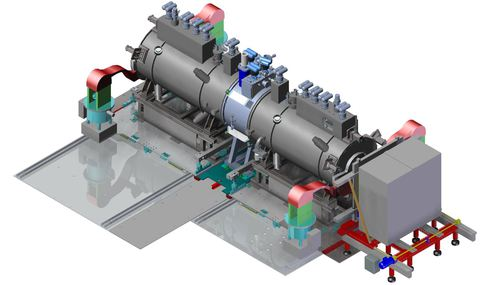
\includegraphics[width=0.9\textwidth]{figs/stepIV-rendering.jpg}
%\caption{Rendering of the next MICE Step IV configuration}
%\end{figure}

\begin{figure}[!htb]
\centering
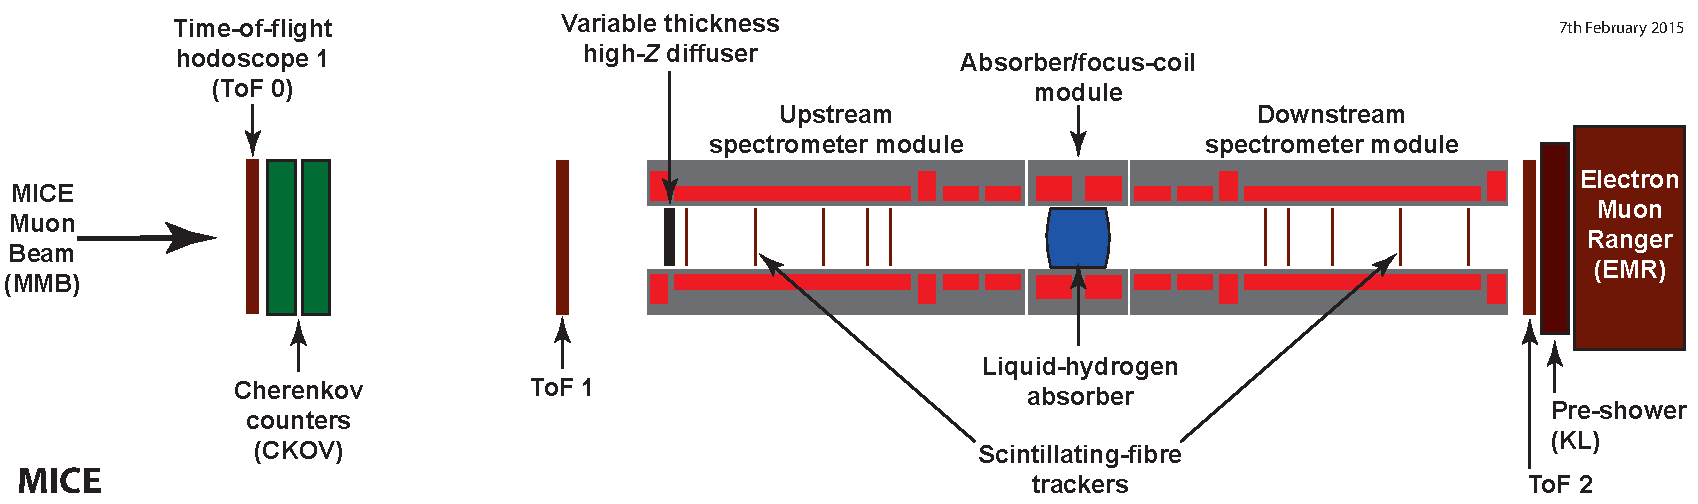
\includegraphics[width=0.9\textwidth]{figs/step4-layout.pdf}
\caption{ Schematic diagram of the final configuration of the MICE experiment. The red rectangles represent the coils of the spectrometer solenoids and focus coil. The individual coils of the spectrometer solenoids are labelled E1, C, E2, M1 and M2. The various detectors are also represented.}
\label{fig:step4}
\end{figure}


\subsection{Software requirements} \label{sec:requirements}

The MICE software must serve both the accelerator-physics and the particle-physics needs of the experiment. Traditional particle-physics functionality includes reconstructing particle tracks, identifying them, and simulating the response from various detectors, while the accelerator-physics aspect includes the calculation of transfer matrices and Twiss parameters and propagating the beam envelopes. All of these require a detailed description of the beamline, the geometries of the detectors, and the magnetic fields, as well as functionality to simulate the various detectors and reconstruct the detector outputs. 

Given the complexity and the time-scale of the experiment, it was essential to ensure that the software can be maintained over the long-term. Good performance was also important in order to ensure that the software can reconstruct data with sufficient speed to support live online monitoring of the experiment.

%\begin{figure}[!htb]
%\centering
%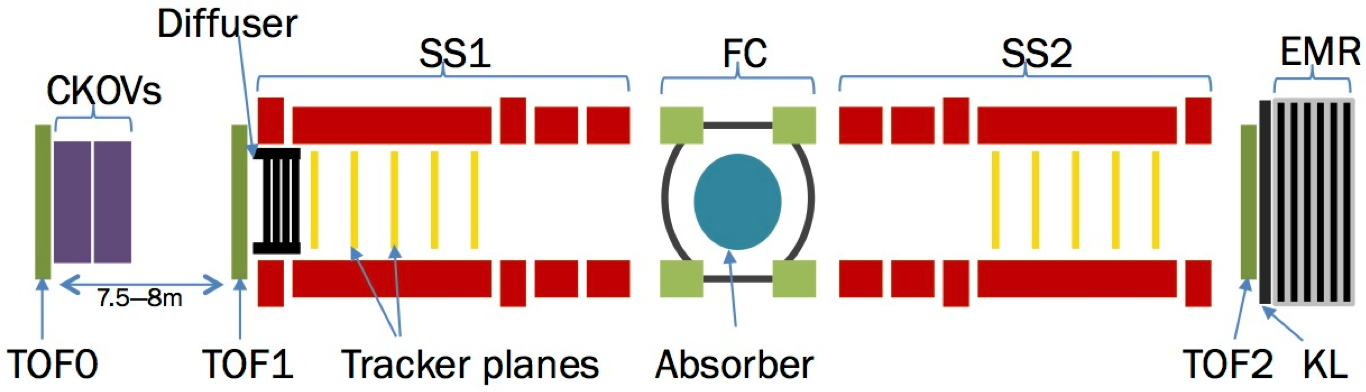
\includegraphics[width=0.9\textwidth]{figs/maus-detectors.png}
%\caption{Sketch of MICE Step IV showing the tracking and particle identification detectors.}
%\label{fig:step4-layout}
%\end{figure}

\section{MAUS}\label{sec:maus}

The MICE  Analysis User Software (MAUS)~\cite{MausIPAC11} is the experiment's simulation, reconstruction, and  analysis software framework. MAUS provides a Monte Carlo (MC) simulation of the experiment, reconstruction of tracks and identification of particles from simulations and real data, and provides monitoring and diagnostics while running the experiment.

Installation is performed via a set of shell scripts with SCons~\cite{SCONS} as the build tool. The codebase is maintained with  the GNU Bazaar revision control system~\cite{bazaar} and is hosted on Launchpad~\cite{launchpad}. MAUS has a number of dependencies on standard packages such as Python, ROOT~\cite{ROOT} and GEANT4~\cite{GEANT4} which are built as "third party" external libraries during the installation process.  The officially supported platform is Scientific Linux 6~\cite{scilinux} though developers have successfully built on CentOS~\cite{centos}, Fedora~\cite{fedora}, and Ubuntu~\cite{ubuntu} distributions.

Each of the MICE detector systems, described in section~\ref{sec:mice}, is represented within MAUS. Their data structures are described in section~\ref{sec:maus-datastr} and their simulation and reconstruction algorithms in sections~\ref{sec:mc, sec:recon}. MAUS also provides ``global'' reconstruction routines, which combine data from individual detector systems to identify particle species by the likelihood method and a global track fit. These algorithms are also described in section~\ref{sec:recon}. 


\subsection{Code design}\label{sec:maus-arch}

MAUS is written in a mixture of Python and C++. C++ is used for complex or low-level algorithms where processing time is important, while Python is used for simple or high-level algorithms where development time is a more stringent requirement. Developers are allowed to write in either Python or C++ and Python bindings to C++ are handled through internal abstractions or SWIG~\cite{SWIG}. In practice, all the reconstruction modules are written in C++ but support is provided for legacy modules written in Python.

MAUS has an Application Programming Interface (API) that provides a framework on which developers can hang individual routines. The MAUS API provides MAUS developers with a well-defined environment for developing reconstruction code, while allowing independent development of the back-end and code-sharing of common elements, such as error handling and data-wrangling. 

The MAUS data processing model is inspired by the Map-Reduce framework~\cite{MapReduce}, which forms the core of the API design. Map-Reduce, illustrated in figure~\ref{fig:mapreduce} is a useful model for parallelizing data processing on a large scale. For MAUS, the API was simplified to use \emph{transformers} in place of maps, though these modules have retained the name \emph{map}. A map process takes a single object as an input, which remains unaltered, and returns a new object as the output, whereas a transformer process alters the input object in place (in the case of MAUS this object is the \emph{spill} class, see Section~\ref{sec:maus-datastr}).

A \emph{Module} is the basic building block of the MAUS API framework. Four types of module exist within MAUS:

\begin{enumerate}
\item \textbf{Inputters} generate input data either by reading data from files or sockets, or by generating an input beam;
\item \textbf{Mappers} modify the input data, for example by reconstructing signals from detectors, or tracking  particles to generate MC hits;
\item \textbf{Reducers} collate the mapped data and allow functionality that requires access to the entire data set; and
\item \textbf{Outputters} save the data  either by streaming over a socket or writing to disk.
\end{enumerate}

\begin{figure}[!htb]
\centering
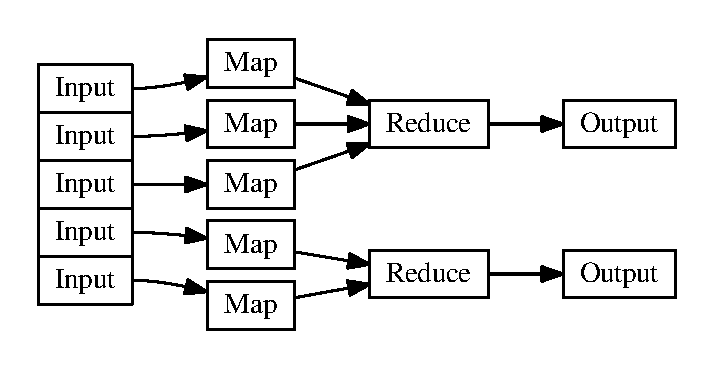
\includegraphics[width=0.7\textwidth]{figs/map_reduce.pdf}
\caption{A Map-Reduce framework.}
\label{fig:mapreduce}
\end{figure}

\noindent Each module type follows a common, extensible, object-orientated class heirarchy, shown for the case of the map and reduce modules in figure~\ref{fig:api}. 

\begin{figure}[!htb]
\centering
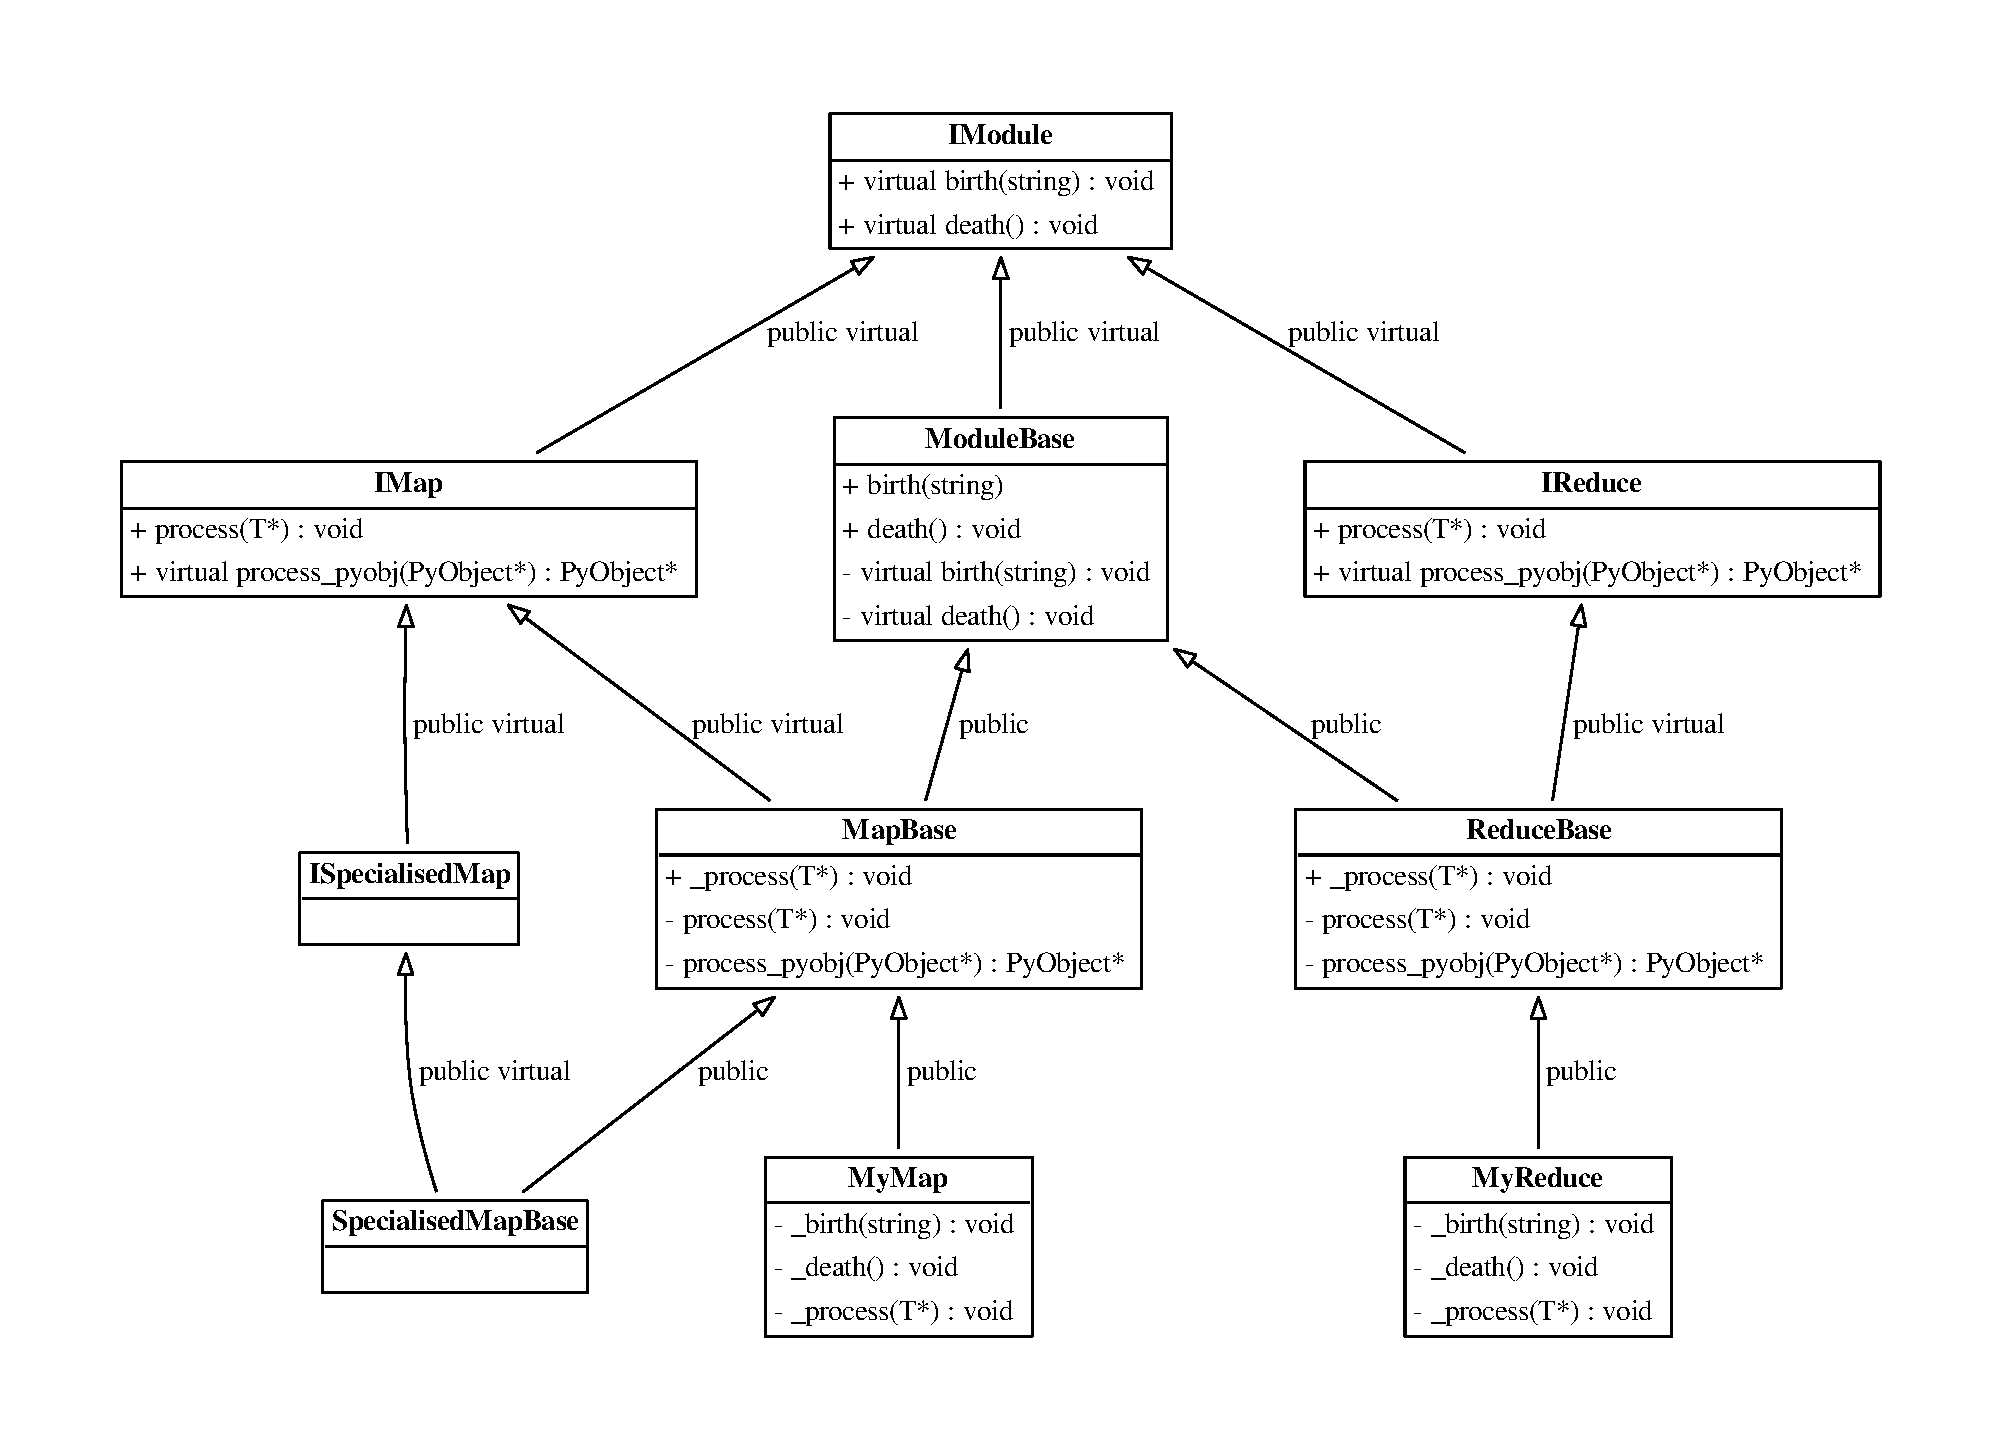
\includegraphics[width=1.0\textwidth]{figs/api.pdf}
\caption{The MAUS API class hierarchy for Map and Reduce modules. The input and output modules follow related designs. \emph{T} represents a templated argument. ``+'' indicates the introduction of a virtual void method, defining an interface, while ``-'' indicates that a class implements that method, fulfilling that aspect of the interface. The  \emph{process\_pyobj} functions are the main entry points for Python applications, and \emph{process} the entry points for C++ applications. The framework can be extended as many times as  necessary, as exemplified by the ``SpecialisedMap'' classes.}
\label{fig:api}
\end{figure}

There are some objects that sit outside the scope of this modular framework but are nevertheless required by several of the modules. For instance,  the detector geometries, magnetic fields, and calibrations are required by the reconsruction and simulation modules, and objects such as the electronics cabling maps are required in order to unpack data from the data acquisition (DAQ) source, and error handling functionality is required by all of the modules. All these objects are accessed through a static singleton \emph{globals} class. 
%After the beginning of the run, mappers can have no internal state, in order to facilitate distributed processing.

MAUS has two execution concepts. A \emph{job} refers to a single execution of the code, while a \emph{run} refers to the processing of data for a DAQ run or MC run. A job may contain many runs. Since data are typically accessed from a single source and written to a single destination, Inputters and Outputters are initialized and destroyed at the beginning and end of a job. On the other hand, Mappers and Reducers are initialized at the beginning of a run in order to allow run-specific information such as electronics cabling maps, fields, and calibrations to be loaded.

The principal data type in MAUS, which is passed from module to module, is the \emph{spill}. A single spill corresponds to  data from the particle burst associated with a dip of the MICE target \cite{BeamlineJINST}. A spill lasts up to $\sim$ 3\,ms and contains several DAQ triggers.  Data from a given trigger define a single MICE \emph{event}. In the language of the Input-Map-Reduce-Output framework, an Input module creates an instance of spill data, a Map module processes the spill (simulating, reconstructing, etc.), a Reduce module acts on a collection of spills when all the mappers finish, and finally an Output module records the data to a given file format.

Modules can exchange spill data either as C++ pointers or JSON~\cite{JSON} objects. In Python, the data format can be changed by using a converter module, and in C++ mappers are templated to a MAUS data type and an API  handles any necessary conversion to that type (see Fig.~\ref{fig:api}). 

%During production deployment of the software it was found that there was a large reduction in processing speed when JSON was used for passing data internally, due to the inherent slowness in (de)serializing each spill to JSON format. Hence it was decided that modules for official reconstruction and simulations must exchange C++ objects by default, in order to minimize need for conversion between data types. However, data can still be output in JSON format and developers find it extremely useful during debugging.

Data contained within the MAUS data structure (see Section~\ref{sec:maus-datastr}) can be saved to permanent storage in one of two formats. The default data format is a ROOT~\cite{ROOT} binary and the secondary format is JSON. ROOT is a standard high-energy physics analysis package, distributed with MAUS, through which many of the analyses on MICE are performed. Each spill is stored as a single entry in a ROOT TTree object.  JSON is an ASCII data-tree format. Specific JSON parsers are available -- for example, the Python \emph{json} library, and the C++ \emph{JsonCpp} \cite{JSONCPP} parser come prepackaged with MAUS. 

In addition to storing the output from the Map modules, MAUS is also capable of storing the data  produced by  \emph{Reducer} modules using a special \emph{Image} class. This class is used by \emph{Reducers} to store images of monitoring histograms, efficiency plots, etc. \emph{Image} data may only be saved in JSON format.

%[??? Clarify ] Besides saving the full data structure, MAUS is also capable outputting the reduced data produced by Reducer modules. These data are not part of the spill, but have their own special data class, known as \emph{Image}. Image is used by Reducers to store images of monitoring histograms, efficiency plots, etc. Image data may only be saved in JSON format.  
%
\subsection{Data structure}\label{sec:maus-datastr}

\subsubsection{Physics data} \label{sec:physics-datastr}

At the top of the MAUS data structure is the spill class which contains all the data from the simulation, raw real data and the reconstructed data. The spill is passed between modules and written to permanent storage. The data within a spill is organized into arrays of three possible event types: an \emph{MCEvent} contains data  representing the simulation of a single particle traversing the experiment and the simulated detector responses; a \emph{DAQEvent} corresponds to the real data for a single trigger; and a \emph{ReconEvent} corresponds to the data reconstructed for a single particle event (arising either from an MC particle or a real data trigger). These different branches of the MAUS data structure are shown diagrammatically in figures~\ref{fig:datastructure-spill}--\ref{fig:datastructure-recon-tof}.

The sub-structure of the the MC event class is shown in figure~\ref{fig:datastructure-mc}. The class is subdivided into events containing detector hits (energy deposited, position, momentum) for each of the MICE detectors (see Section~\ref{sec:mice}). The event also contains information about the primary particle that created the hits in the detectors.

The sub-structure of the the reconstruction event class is shown in figure~\ref{fig:datastructure-recon}. The class is subdivided into events representing each of the MICE detectors, together with the data from the trigger, and data for the global event reconstruction. Each detector class and the global reconstruction class has several further layers of reconstruction data. This is shown in figures~\ref{fig:datastructure-recon-ckov-emr-kl}--\ref{fig:datastructure-recon-tof}.

\begin{figure}[!p]
\centering
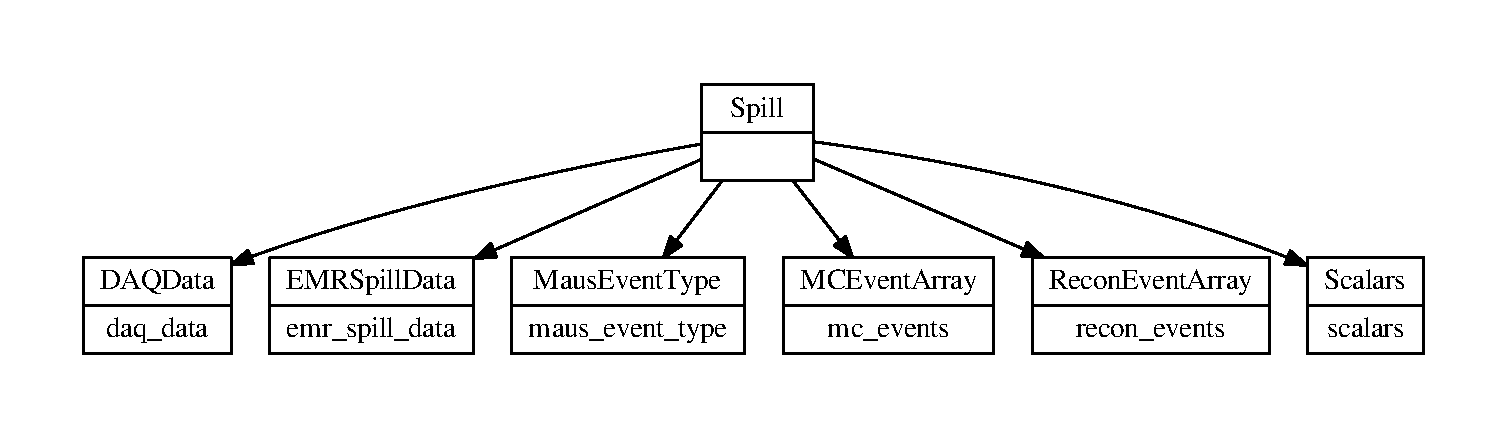
\includegraphics[width=\textwidth]{figs/spill_datastructure.pdf}
\caption{The MAUS output structure for a spill event. The top label in each box is the name of the C++ class and the bottom label is the json branch name.}
\label{fig:datastructure-spill}
\end{figure}

\begin{figure}[ptb]
\centering
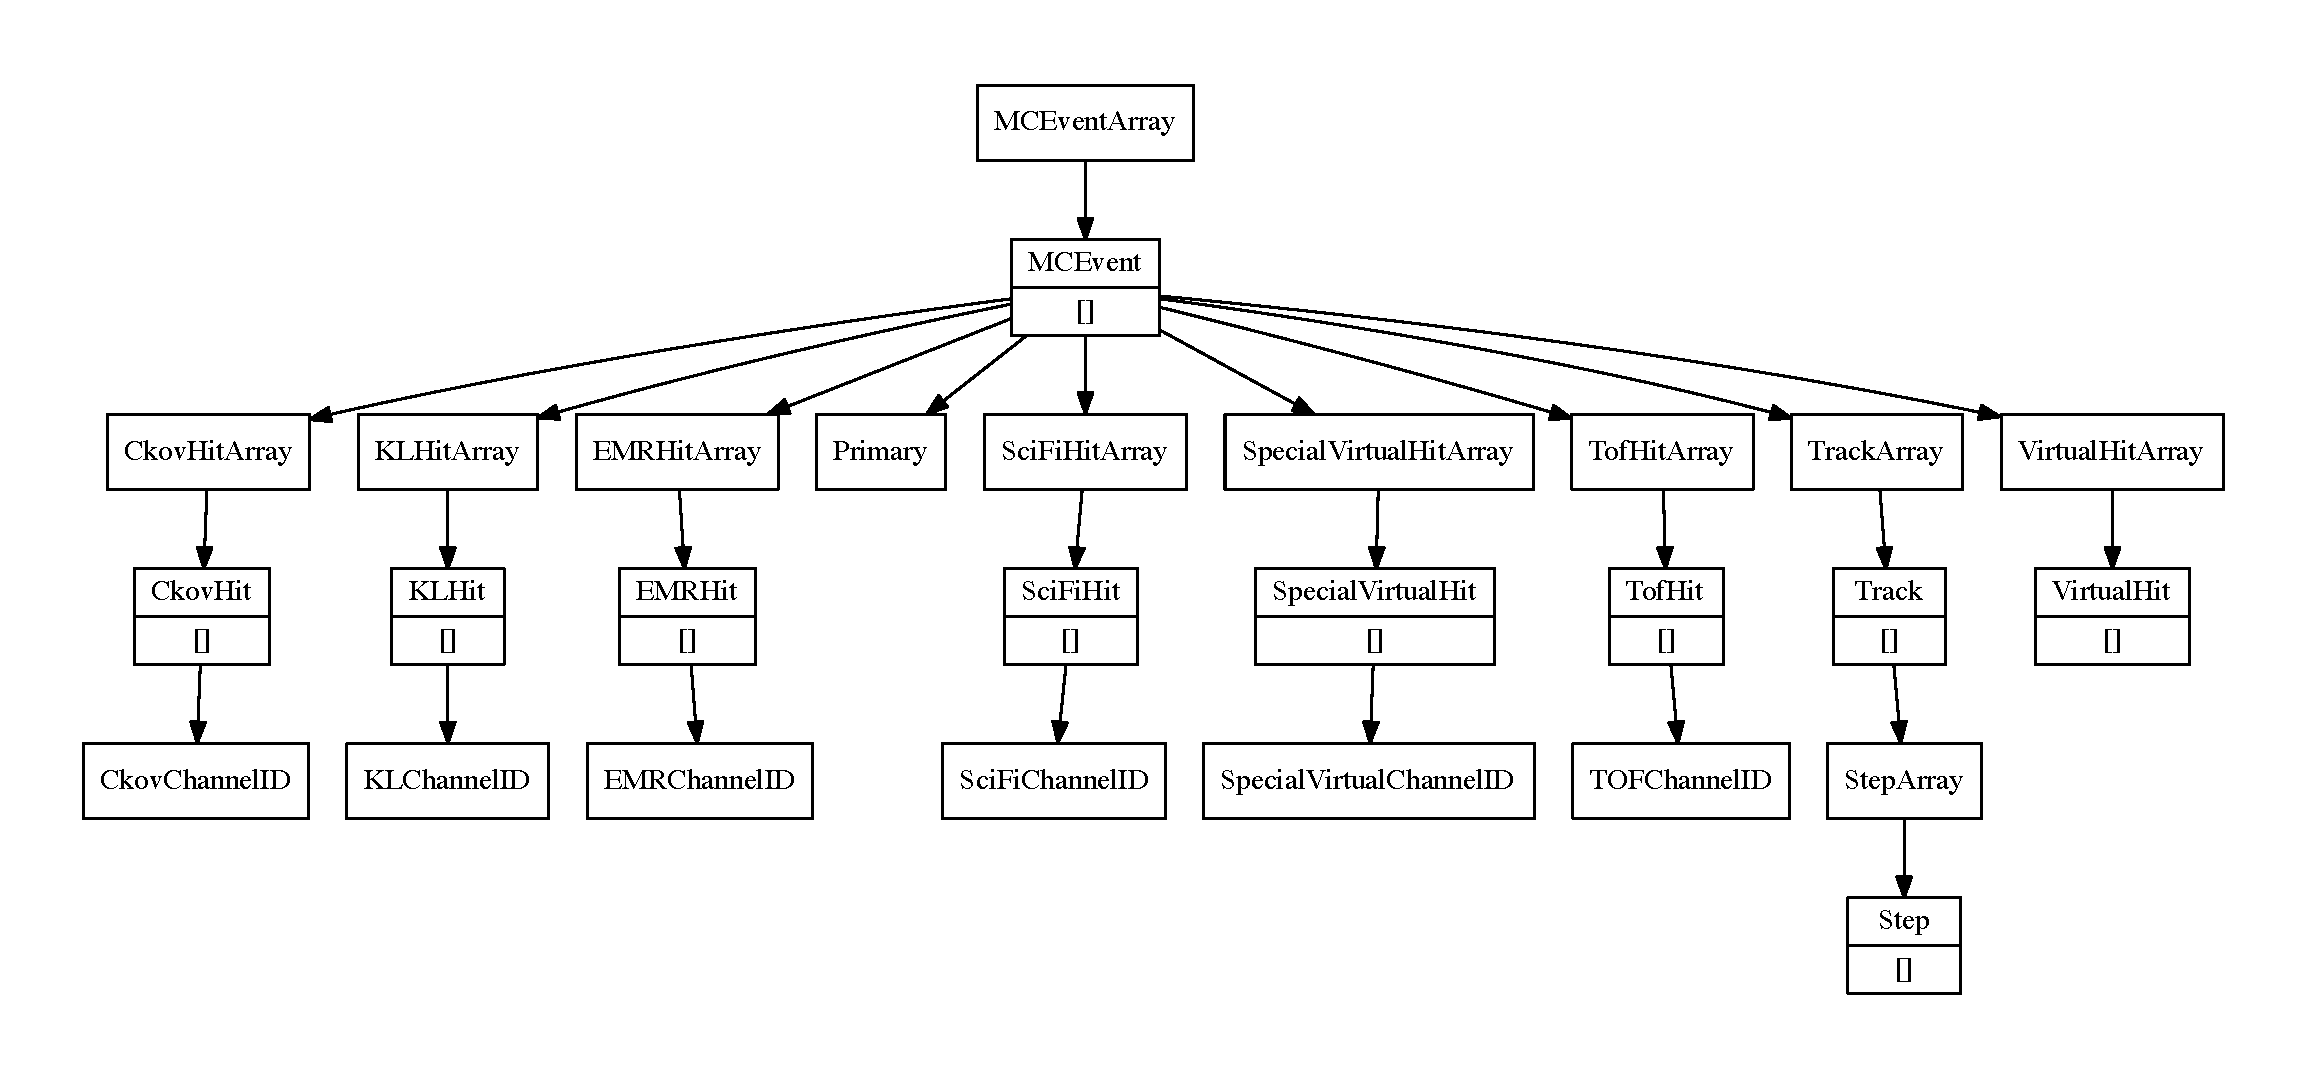
\includegraphics[width=\textwidth]{figs/mc_datastructure.pdf}
\caption{The MAUS data structure for MC events. The top label in each box is the name of the C++ class and the bottom label is the json branch name. [] indicates that child objects are array items.}
\label{fig:datastructure-mc}
\end{figure}

\begin{figure}[ptb]
\centering
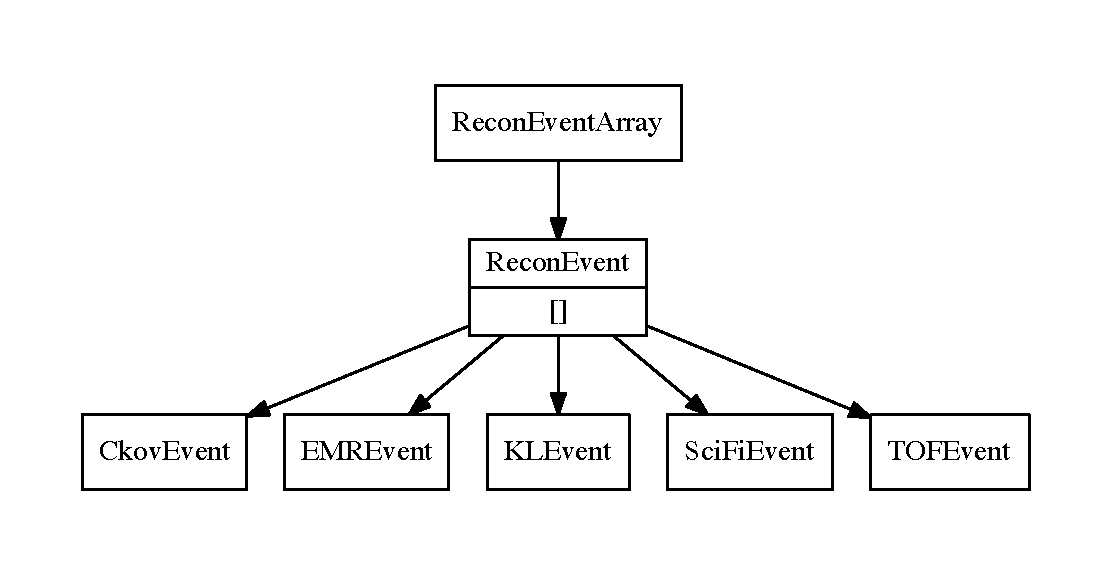
\includegraphics[width=\textwidth]{figs/recon_datastructure.pdf}
\caption{The MAUS data structure for reconstructed events. The top label in each box is the name of the C++ class and the bottom label is the json branch name.}
\label{fig:datastructure-recon}
\end{figure}

\begin{figure}[ptb]
\centering
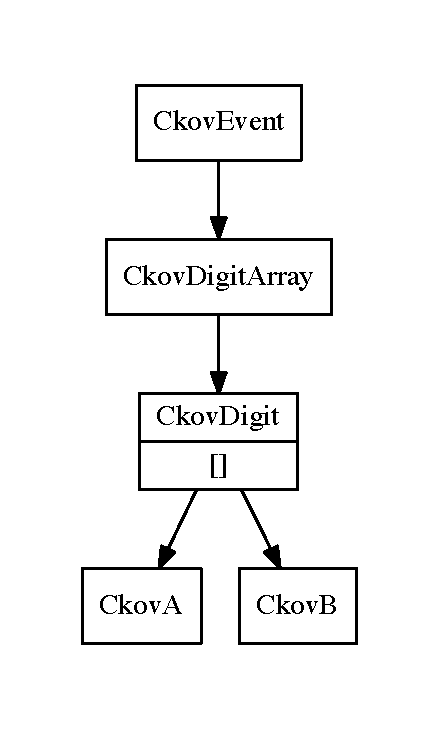
\includegraphics[width=0.3\textwidth]{figs/ckov_datastructure.pdf}
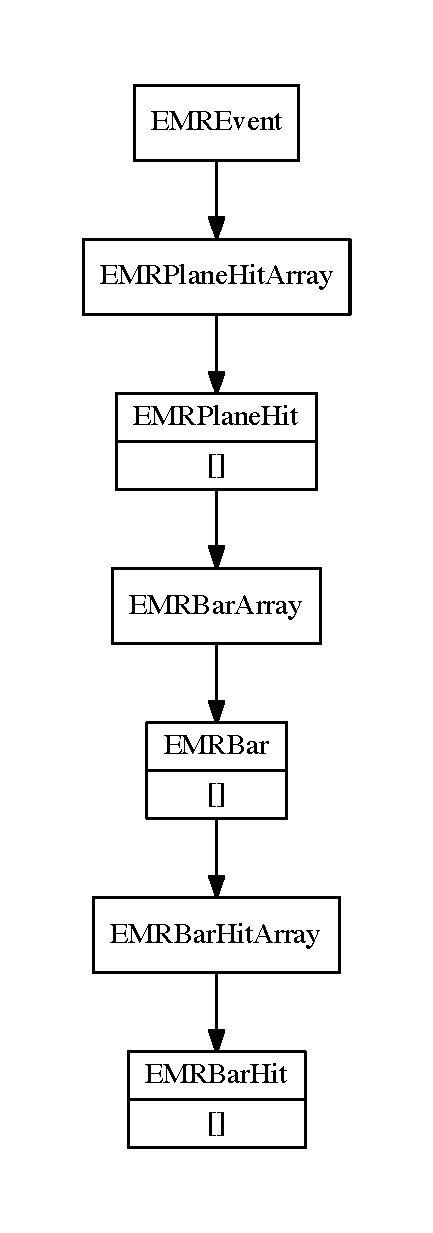
\includegraphics[width=0.25\textwidth]{figs/emr_datastructure.pdf}
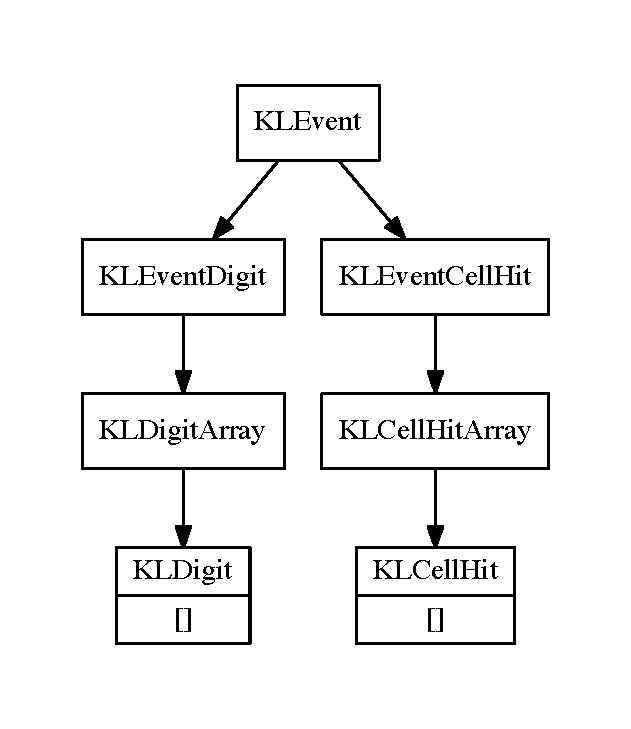
\includegraphics[width=0.4\textwidth]{figs/kl_datastructure.pdf}
\caption{The MAUS data structure for CKOV (left), EMR (middle) and KL (right) reconstructed events. The top label in each box is the name of the C++ class and the bottom label is the json branch name. [] indicates that child objects are array items.}
\label{fig:datastructure-recon-ckov-emr-kl}
\end{figure}

\begin{figure}[ptb]
\centering
%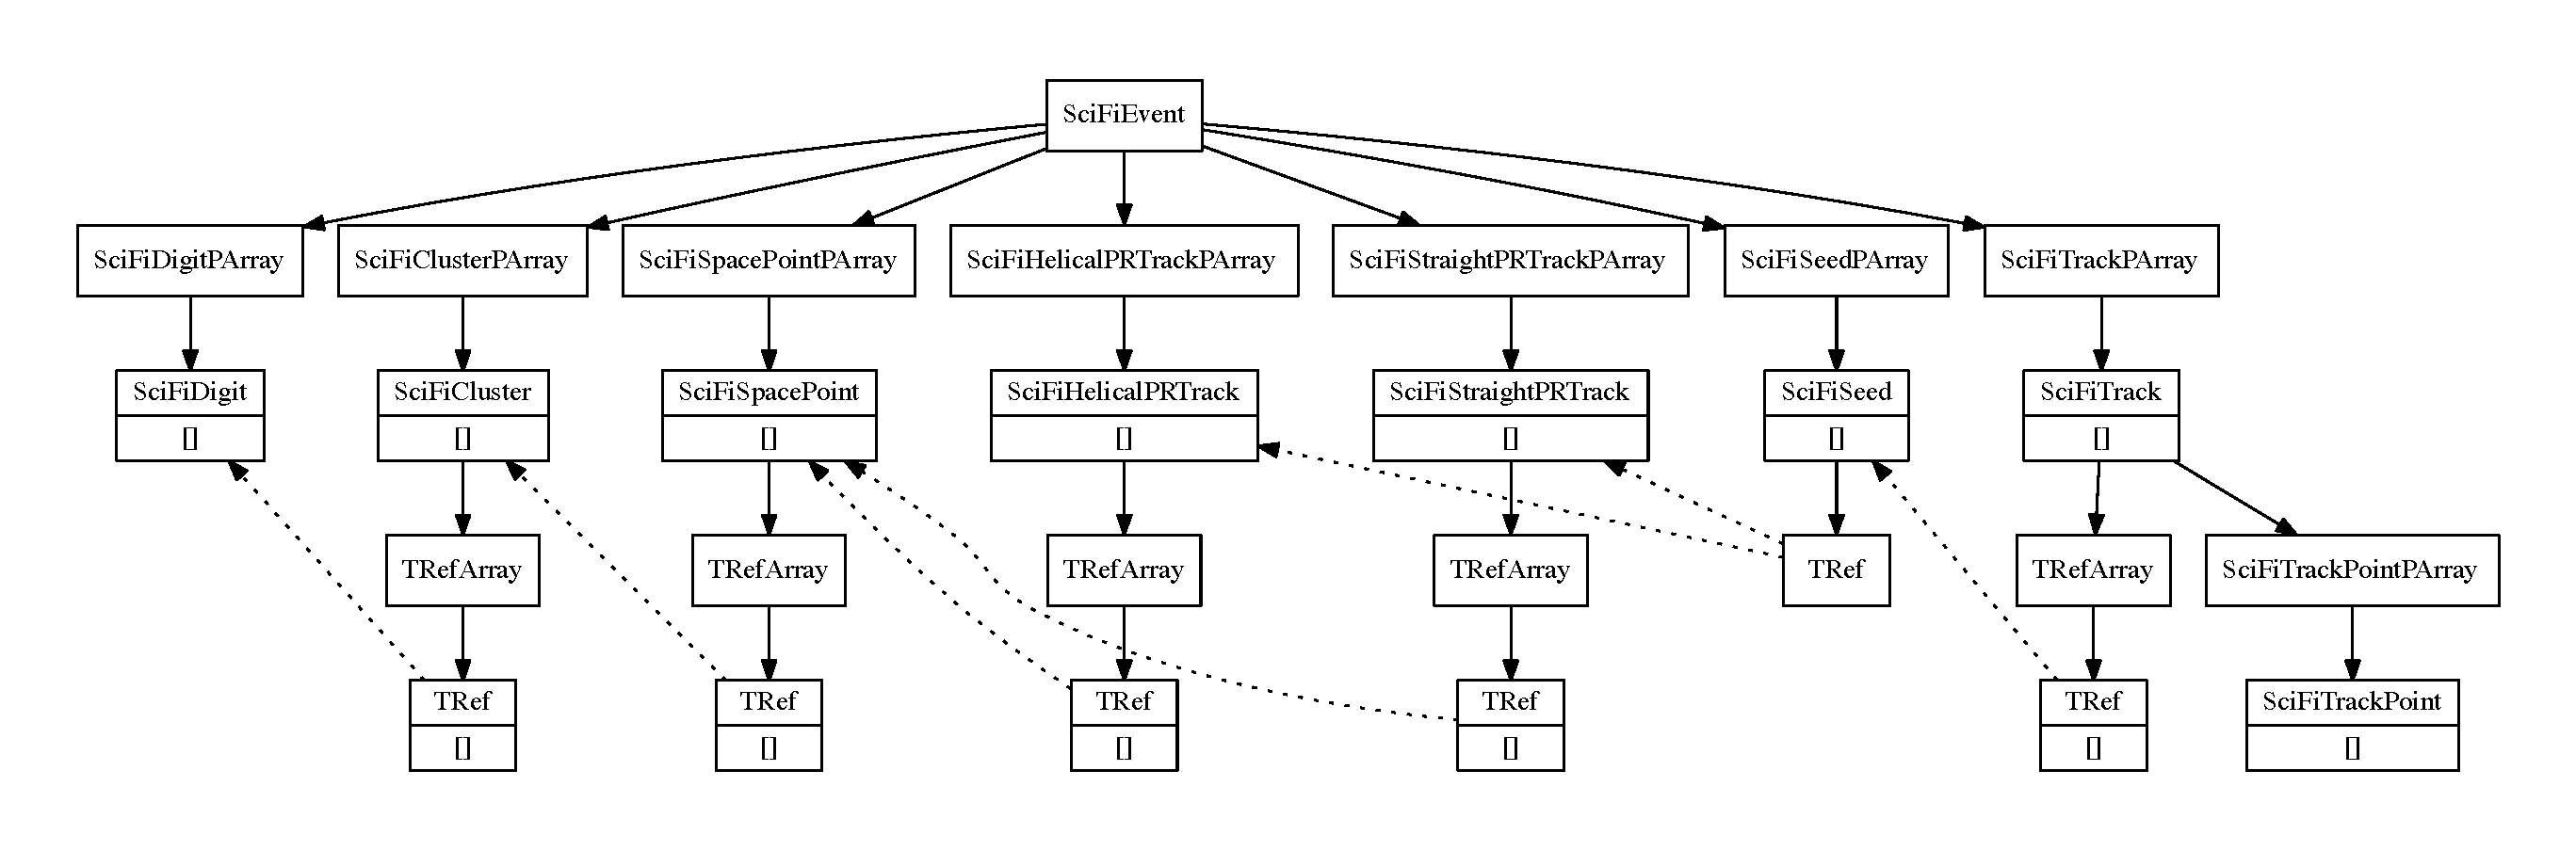
\includegraphics[width=1.0\textwidth]{figs/scifi_datastructure.pdf}
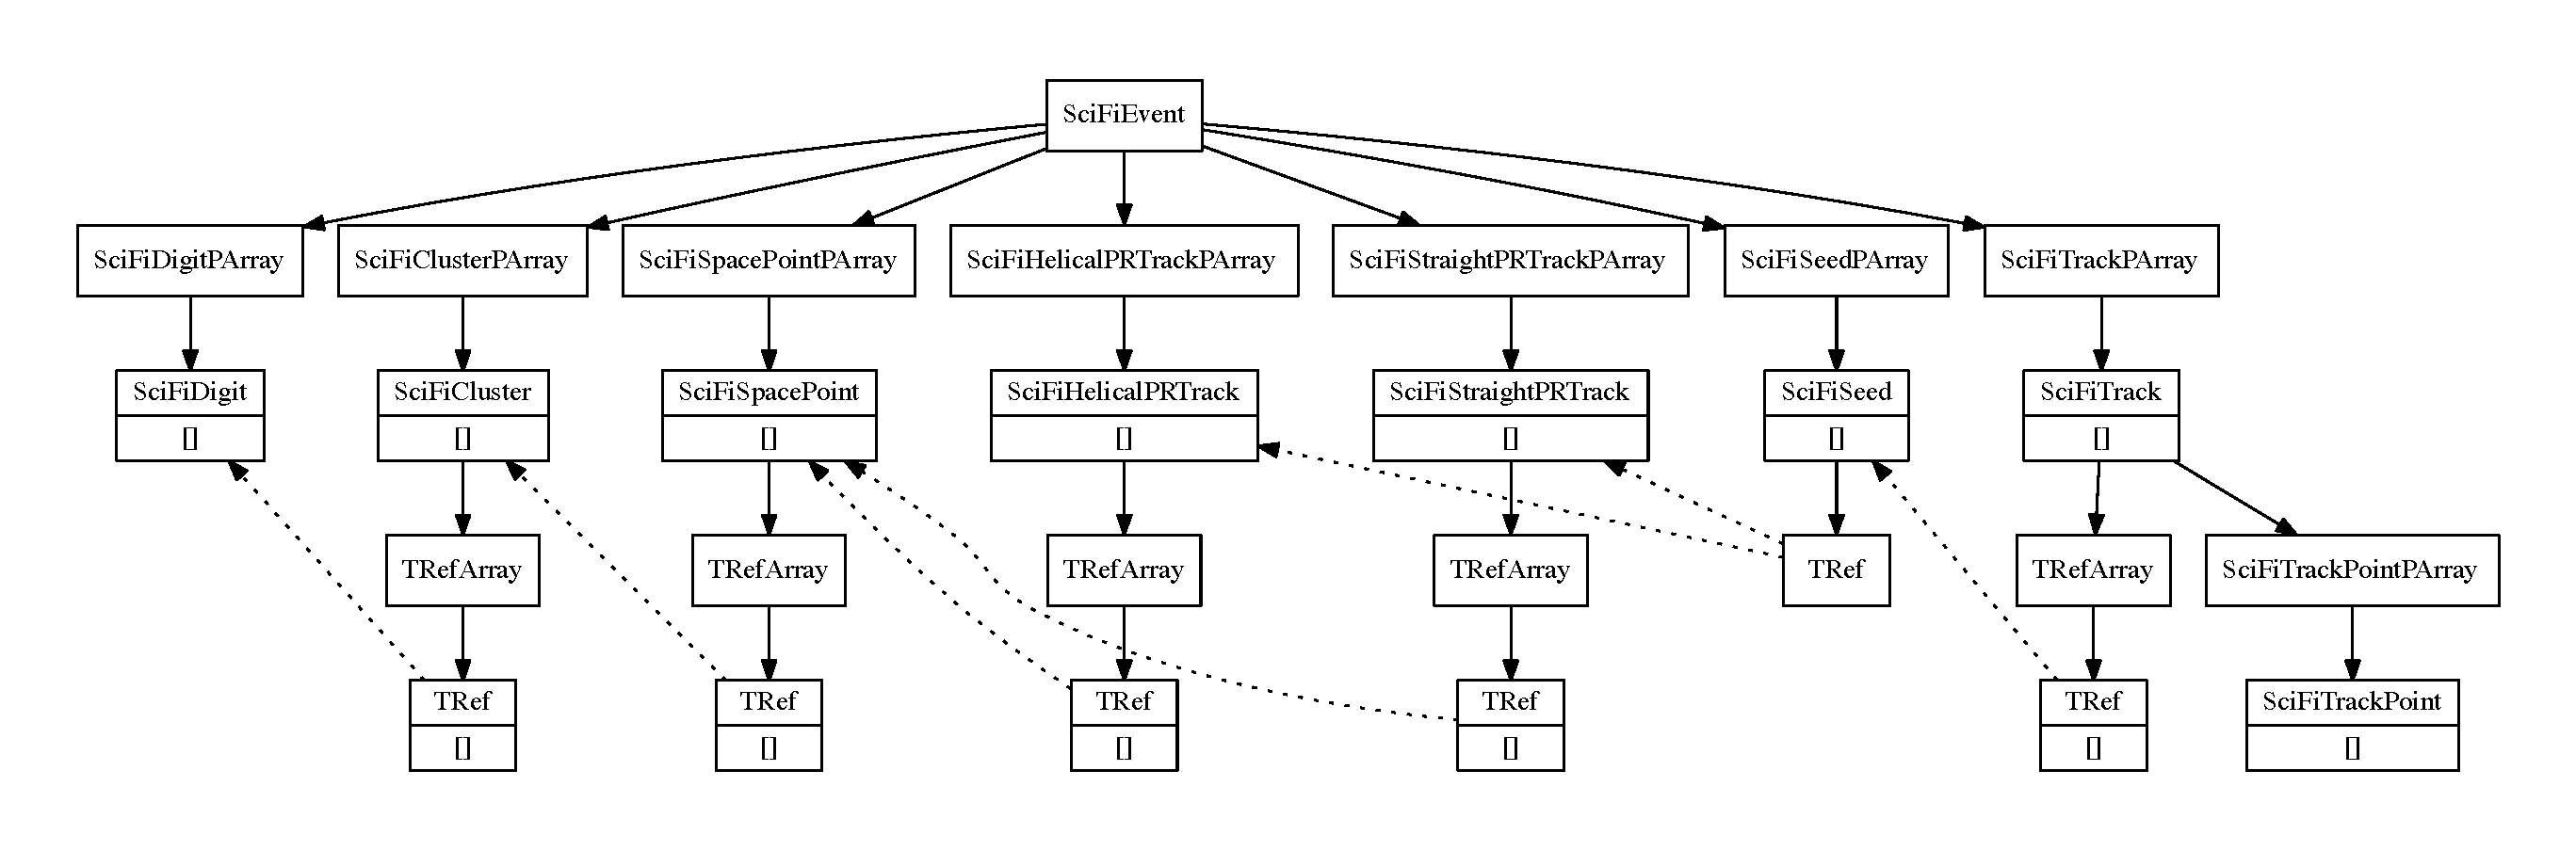
\includegraphics[width=1.0\textheight,angle=90,origin=c]{figs/scifi_datastructure.pdf}
\caption{The MAUS data structure for the tracker. The top label in each box is the name of the C++ class and the bottom label is the json branch name. []  indicates that child objects are array items.}
\label{fig:datastructure-recon-scifi}
\end{figure}

\begin{figure}[ptb]
\centering
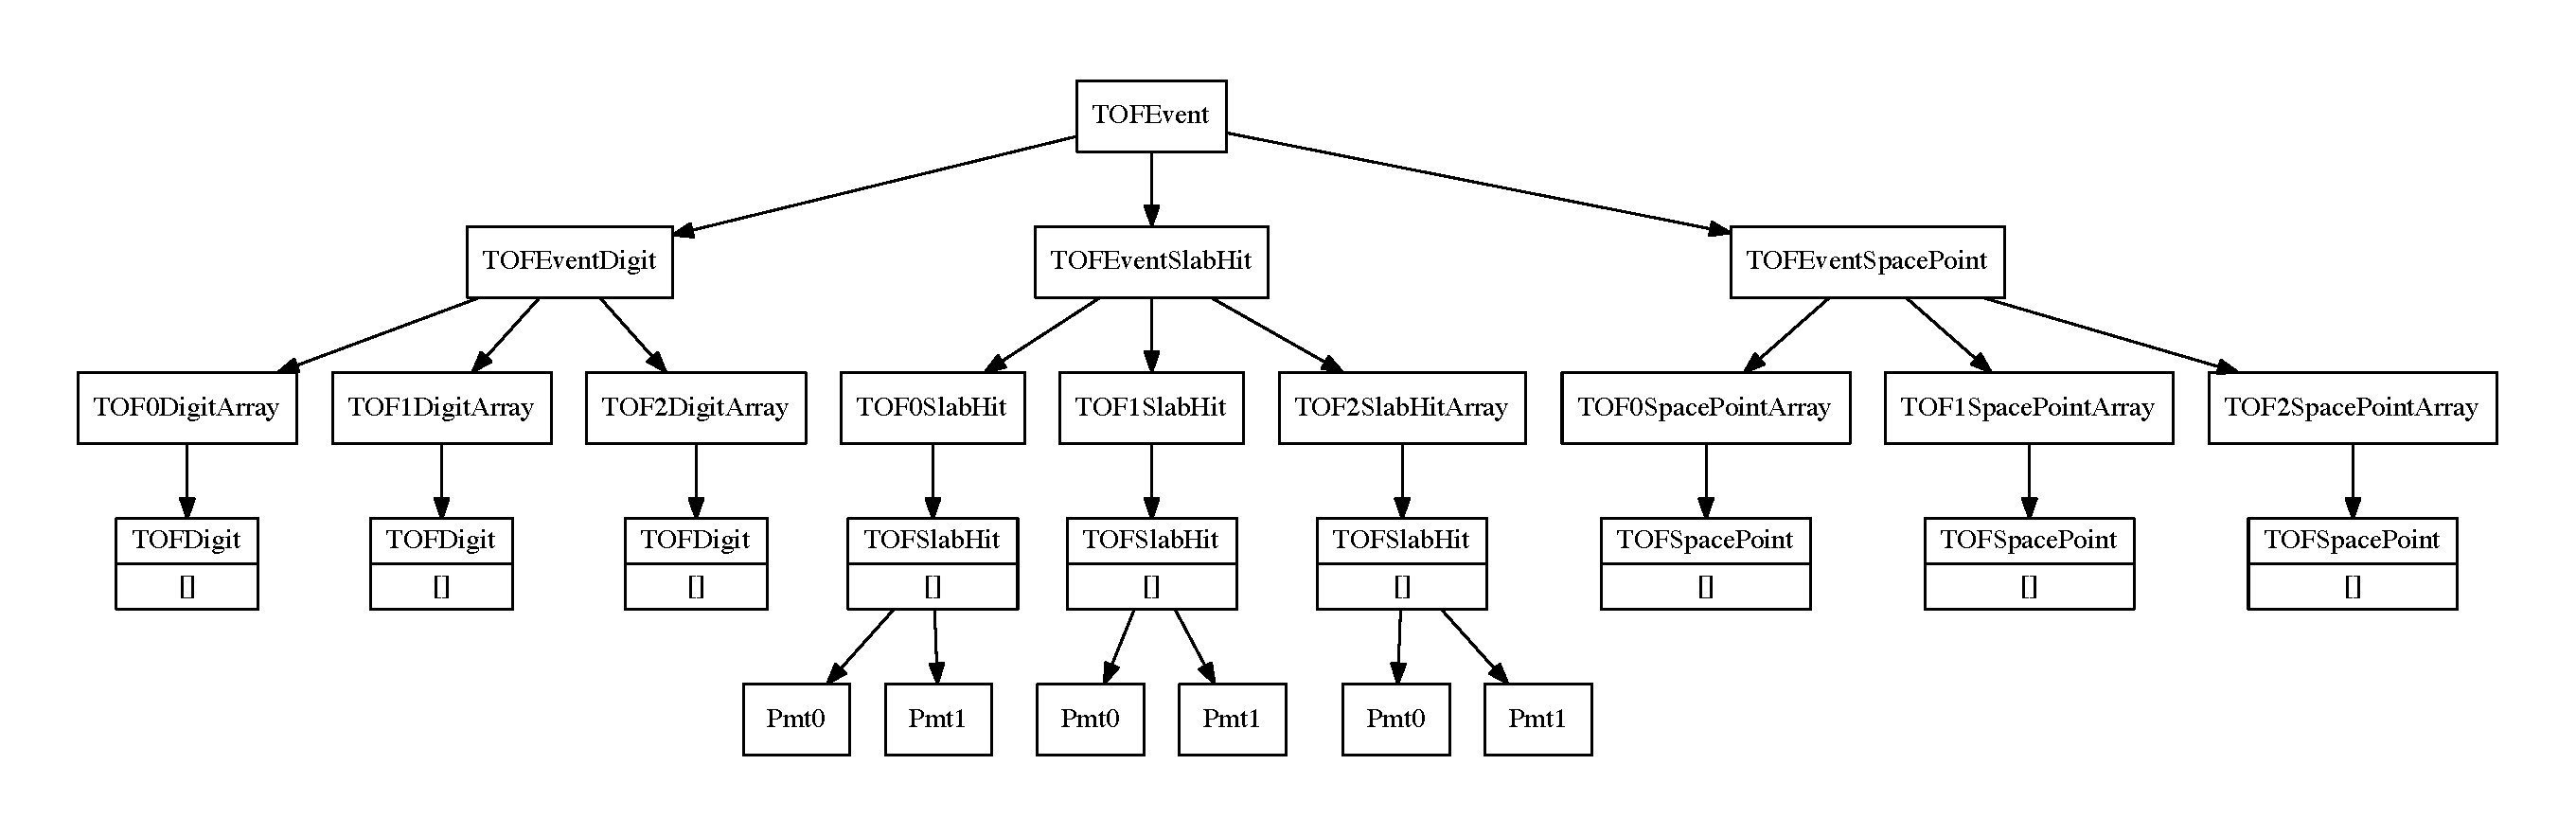
\includegraphics[width=1.0\textwidth]{figs/tof_datastructure.pdf}
\caption{The MAUS data structure for the TOFs. The top label in each box is the name of the C++ class and the bottom label is the json branch name. [] indicates that child objects are array items.}
\label{fig:datastructure-recon-tof}
\end{figure}

\FloatBarrier

\subsubsection{Top level data organisation} \label{sec:top-level-datastr}

In addition to the spill data, MAUS also contains structures for storing supplementary information for each run and job. These are referred to as \emph{JobHeader} and \emph{JobFooter}, and \emph{RunHeader} and \emph{RunFooter}. The former represents data from the start and end of a job, such as the MAUS release version used to create it, and the latter data from the start and end of a run, such as the geometry ID used for the data processing. This may be saved to permanent storage along with the spill.

In order to interface with ROOT, particularly in order to save data in the ROOT format, thin wrappers for each of the top level classes, and a templated base class, were introduced. This allows the ROOT TTree, in which the output data is stored (see Section~\ref{sec:physics-datastr}), to be given a single memory address to read from. The wrapper for Spill is called \emph{Data}, while for each of RunHeader, RunFooter, JobHeader and JobFooter, the respective wrapper class is just given the original class name with ``Data'' appended, e.g., \emph{RunHeaderData}. The base class for each of the wrappers is called \emph{MAUSEvent}. The class hierarchy is illustrated in Figure~\ref{fig:top-level}.

\begin{figure}[htb]
\centering
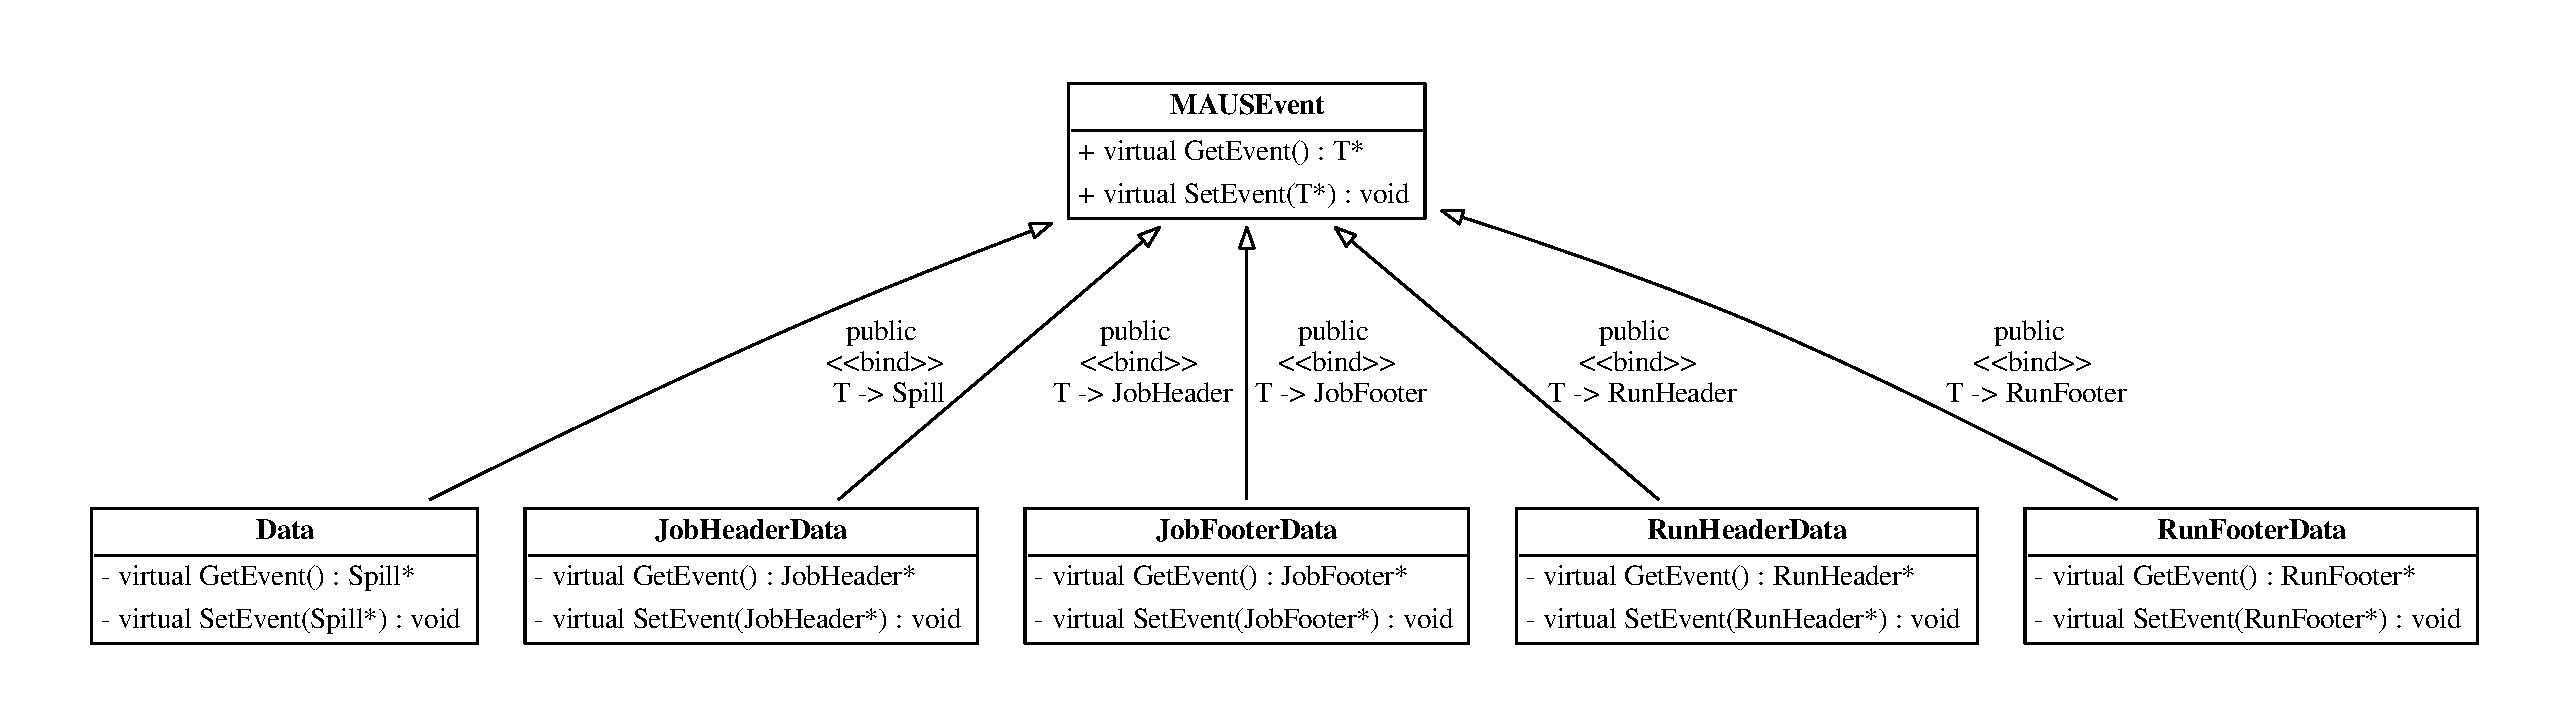
\includegraphics[width=1.03\textwidth]{figs/top_level.pdf}
\caption{Class hierarchy for the wrappers and base class of the top-level classes of the MAUS data structure.}
\label{fig:top-level}
\end{figure}

\subsection{Data flow}\label{sec:maus-dataflow}

The MAUS data flow, showing the reconstruction chain for data originating from MC or real data, is depicted in figure~\ref{fig:maus_process_diagram}. Each item in the diagram is implemented as an individual module. The data flow is grouped into three principal areas: the simulation data flow used to generate digits (electronics signals) from particle tracking; the real data flow used to generate digits from real detector data; and the reconstruction data flow which illustrates how digits are built into higher level objects and converted to parameters of interest. The reconstruction data flow is the same for digits from real data and simulation.  In the case of real data, separate input modules are provided to read either directly from the DAQ, or from archived data stored on disk. A reducer module for each detector provides functionality to create summary histograms.


\begin{figure}[htbp]
  \centering
   %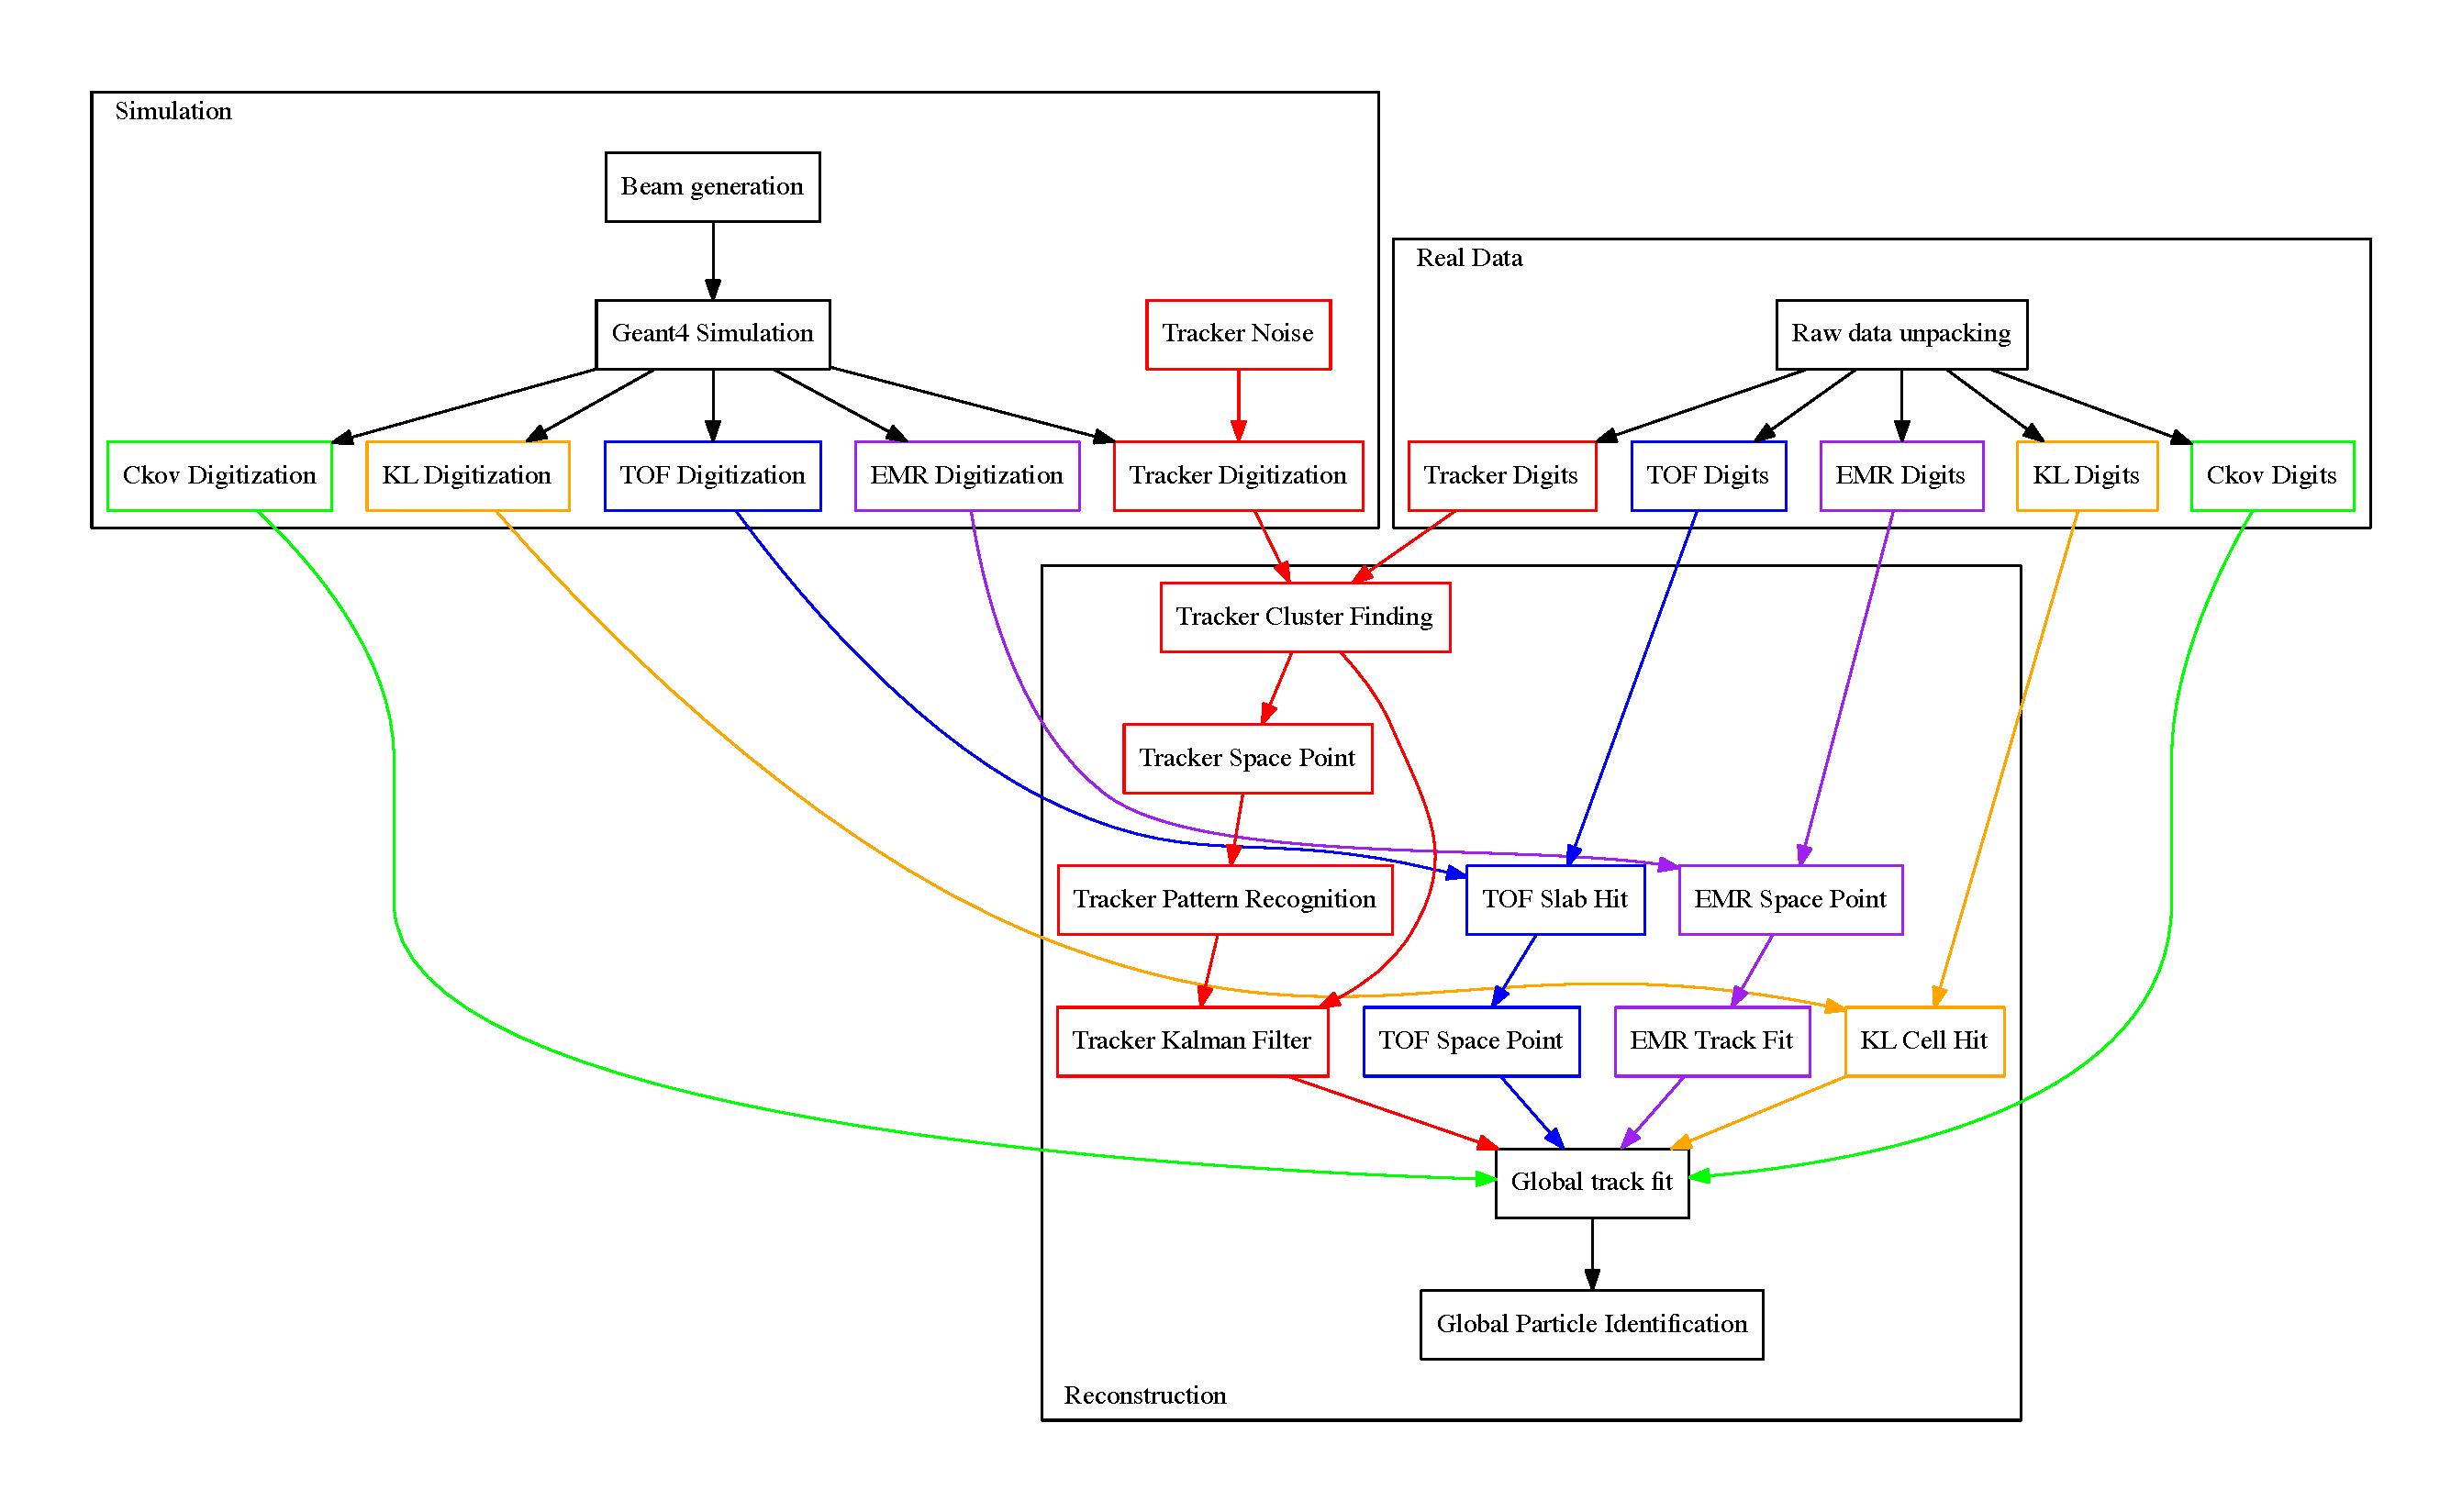
\includegraphics[width=1.0\textwidth]{figs/maus_process_diagram.pdf}
  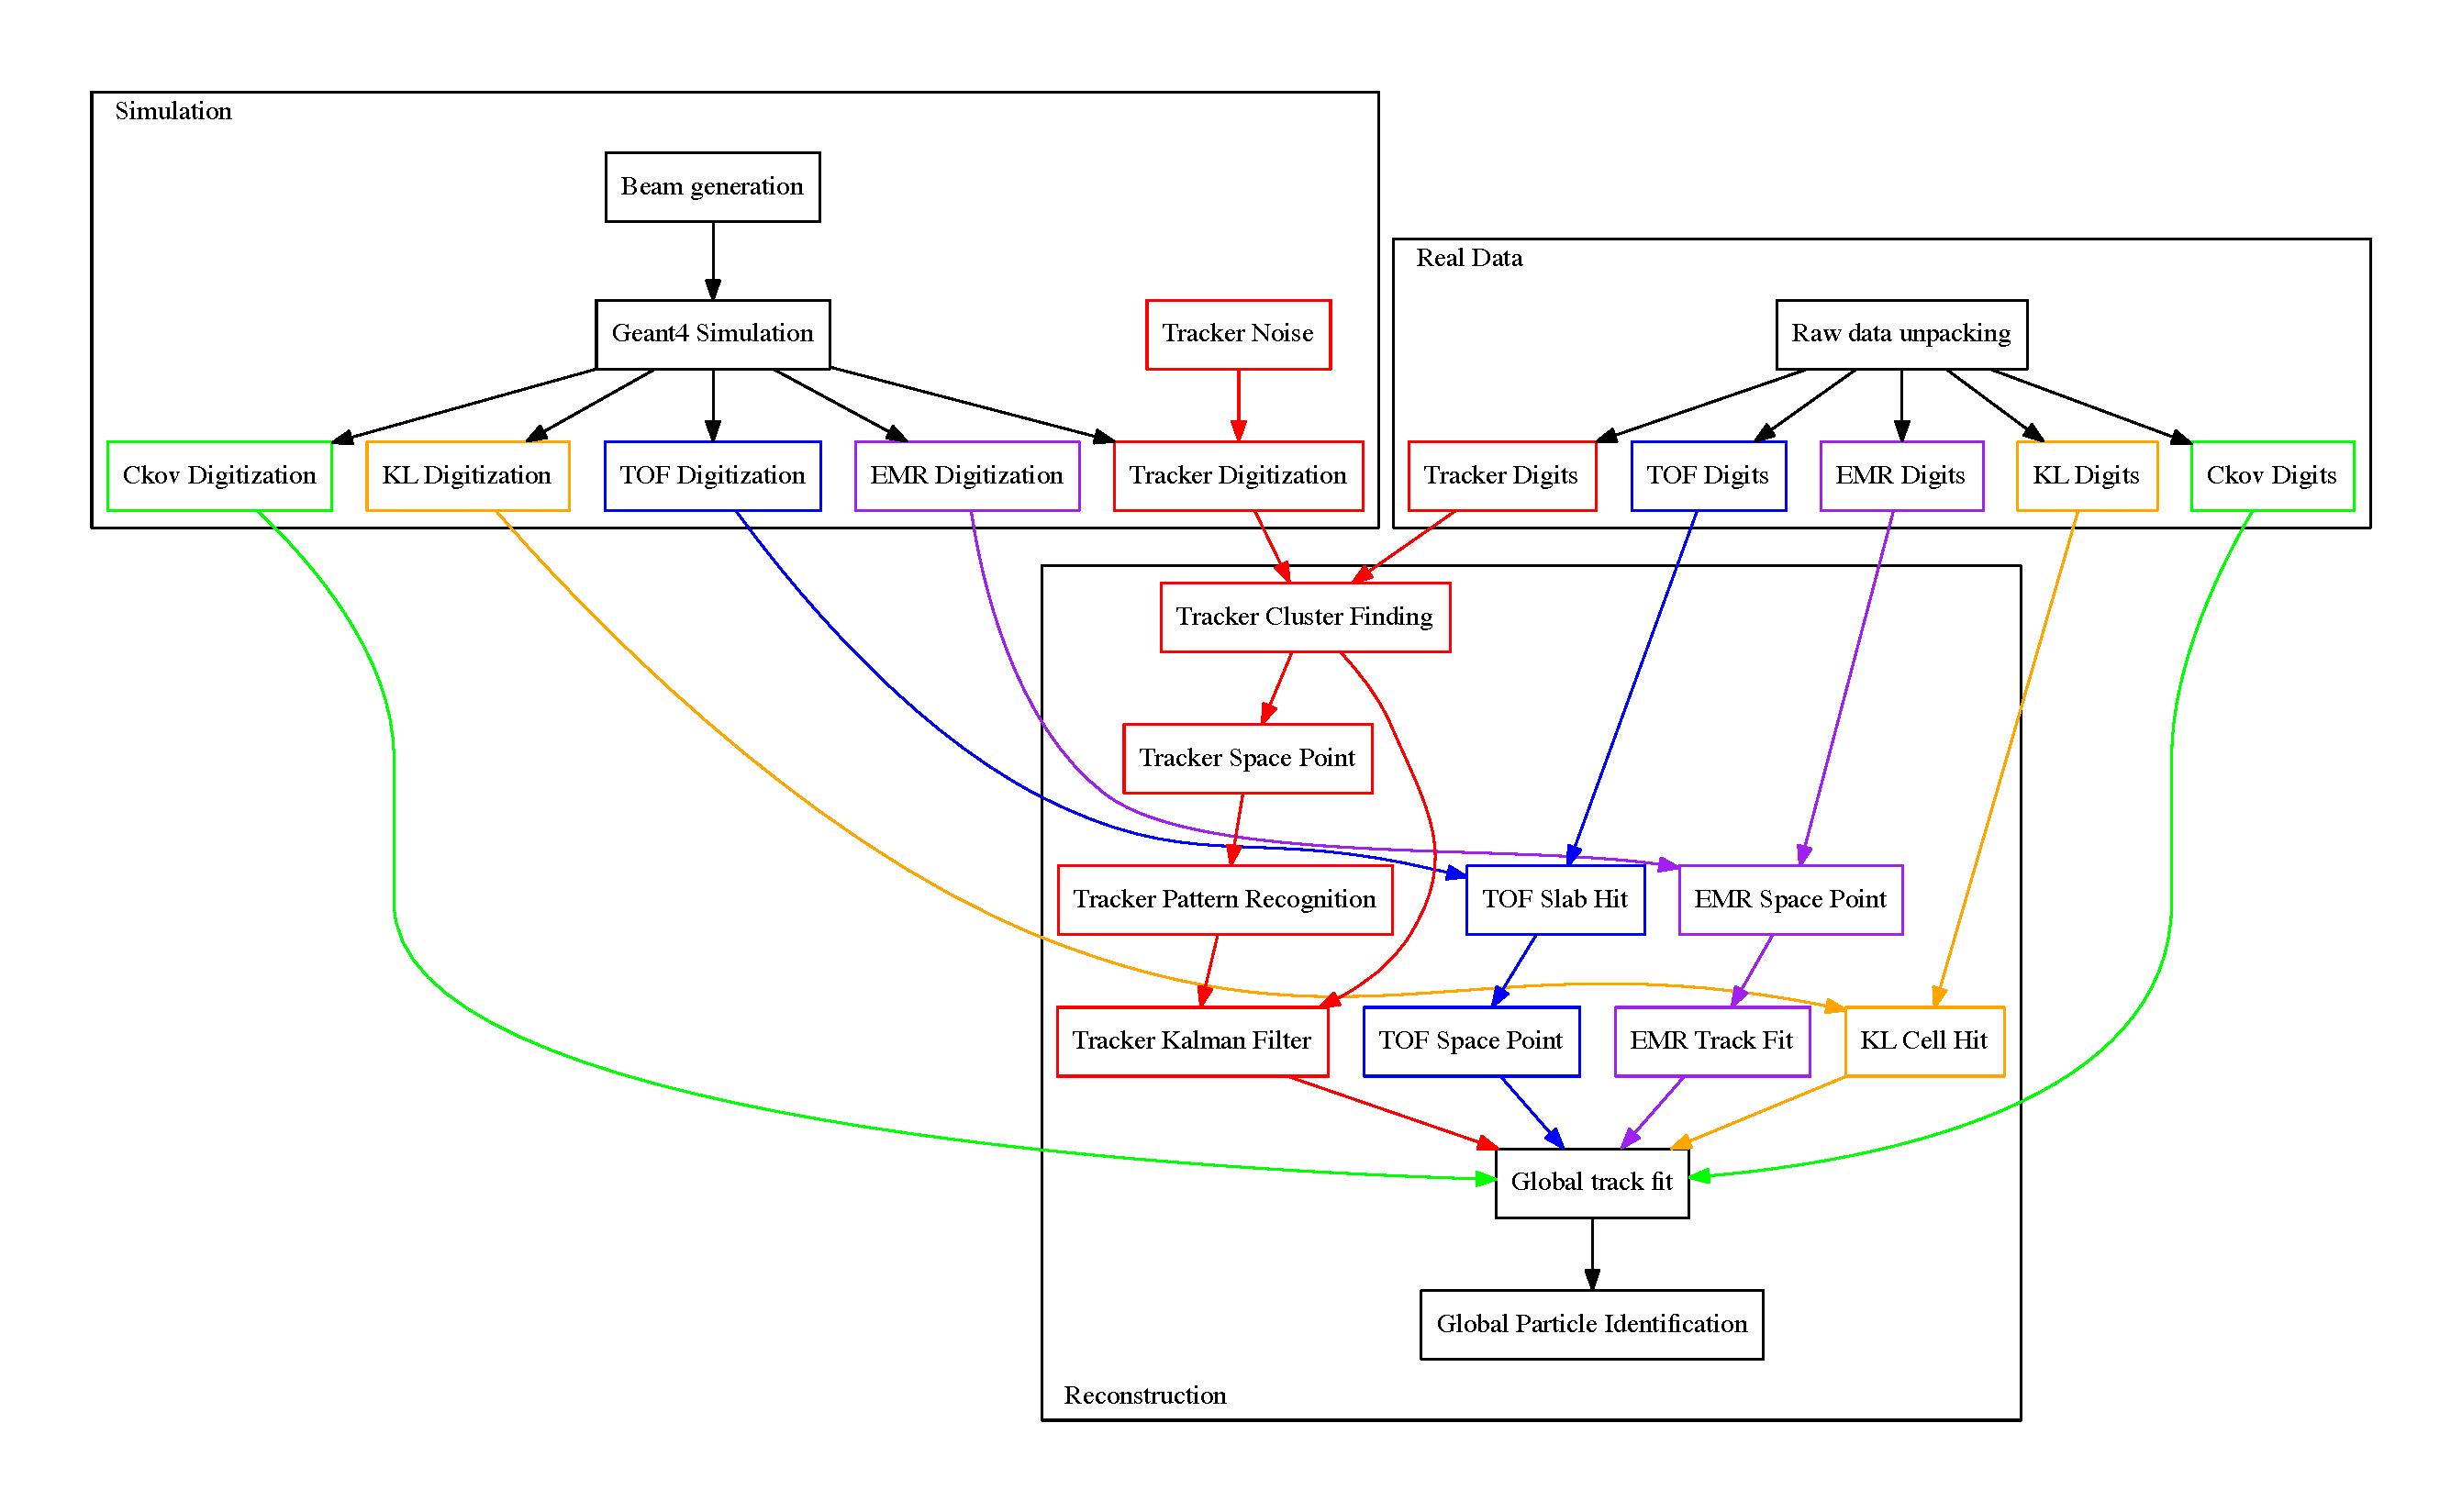
\includegraphics[width=0.9\textheight, angle=90, origin=c]{figs/maus_process_diagram.pdf}
  \caption{Data flow for the MAUS project. The data flow is color-coded by detector: Ckov - green, EMR - purple, KL - orange, TOF - blue, Tracker - red. }
  \label{fig:maus_process_diagram}
\end{figure}

\subsection{Testing}\label{sec:maus-tests}
MAUS has a set of tests at the unit level and the integration level, together with code-style tests for both Python and C++. Unit tests are implemented to test a single function, while integration tests operate on a complete workflow. Unit tests check that each function operates as intended by the developer and achieve a high level of code coverage and good test complexity. Integration tests allow the overall performance of the code to be checked against specifications. The MAUS team provides unit test coverage that executes 70--80 $\%$ of the total code base. This level of coverage typically results in a code that performs the major workflows without any problem.
%
%but has errors in some of the less well-used functions and can behave ungracefully following user error. At the most recent release, MAUS  test coverage was  68 $\%$ for python code, 78 $\%$ for non-legacy C++ code and 36 $\%$ for legacy (pre-2011) C++ code.

The MAUS codebase is built and tested using a Jenkins~\cite{Jenkins} continuous integration environment deployed on a cluster of servers. Builds and tests of the development branch are automatically triggered when there is a change to the codebase.  Developers are asked to perform a build and test on a personal branch of the codebase using the test server before requesting a merge with the development trunk. This enables the MAUS team to make frequent clean releases. Typically MAUS works on a 4--8 week major-release cycle.

%MAUS operates a continuous integration stack using a suite of test servers. Code-building and testing is driven by the Jenkins test environment~\cite{Jenkins}. Developers are asked to perform a build and test on a personal branch of the code-base using the test server before requesting a merge with the development trunk. This enables the MAUS team to make frequent clean releases. Typically MAUS works on a 4--8 week major-release cycle.

\section{Monte Carlo}\label{sec:mc}
A Monte Carlo simulation of MICE encompasses beam generation, geometrical description of detectors  and fields, tracking of particles through detectors and digitization of the detectors' response to particle interactions. 

\subsection{Beam generation}\label{sec:beam}
Several options are provided to generate an incident beam.  Routines are provided to sample particles from a multivariate Gaussian distribution or generate ensembles of identical particles (pencil beams). In addition, it is possible to produce time distributions that are either rectangular or triangular in time to give a simplistic representation of the MICE time distribution. Parameters, controlled by datacards, are available to control random seed generation,  relative weighting of particle species and the transverse-to-longitudinal coupling in the beam. MAUS also allows the generation of a polarized beam. 

Beam particles can also be read in from an external file created by G4Beamline \cite{G4Beamline} or ICOOL \cite{ICOOL}, as well as files in user-defined formats. In order to generate beams which are more realistic taking into account the geometry and fields of the actual MICE beamline, we use G4Beamline to model the MICE beamline from the target to a point upstream of the second quad triplet (upstream of Q4).  The beamline settings, \textit{e.g.,} magnetic field strengths and number of particles to generate, are controlled through data-cards. The magnetic field strengths have been tuned to produce beams that are reasonably accurate descriptions of the real beam. Scripts to install G4beamline are shipped with MAUS. 

Once the beam is generated, the tracking and interactions of particles as they traverse the rest of the beamline and the MICE detectors  is performed using GEANT4.

\subsection{Geant4}\label{sec:geant}
The MICE Muon Beam line consists of a quadrupole triplet that captures pions produced when the MICE target intersects the ISIS proton beam, a pion-momentum-selection dipole, a superconducting solenoid to focus and transport the particles to a second dipole that is used to select the muon-beam momentum and a transport channel composed of a further two quadrupole triplets. The GEANT4 simulation within MAUS starts 1\,m downstream of the second beamline dipole magnet (D2). GEANT4 bindings are encoded in the Simulation module. GEANT4 groups particles by run, event and track. A GEANT4 run maps to a MICE spill; a GEANT4 event maps to a single inbound particle from the beamline; and a GEANT4 track corresponds to a single particle in the experiment.

GEANT provides a variety of reference physics processes to model the interactions of particles with matter. The default process in MAUS is ``\emph{QGSP\_BERT}'' which causes GEANT4 to model hadron interactions using a Bertini cascade model up to 10 GeV/$c$. MAUS provides methods to set up the GEANT4 physical processes through user-controlled data-cards. Finally, MAUS provides routines to extract particle data from the GEANT tracks at user-defined locations.

\subsection{Geometry}\label{sec:geo}

MAUS uses an online Configuration Database to store all of its
geometries. These geometries have been extracted from CAD drawings
which are  updated based on the most recent surveys and technical drawings
available. The CAD drawings are translated to a geometry-specific
subset of XML, the Geometry Description Markup Language (GDML)~\cite{GDML} prior
to being recorded in the configuration database through the use of the 
FastRAD~\cite{fastrad} commercial software package. 

The GDML formatted description contains the beamline elements and the positions of
the detector survey points. Beam-line elements are described using 
tessellated solids to define the shapes of the physical
volumes. The detectors themselves are described using an independently
generated set of GDML files using GEANT4 standard volumes. An
additional XML file is appended to the geometry description that
assigns magnetic fields and associates the detectors to their
locations in the GDML files. This file is
initially written by the geometry maintainers and formatted to contain
run-specific information during download.

The GDML files can be read via a
number of  libraries in Geant4 and ROOT for the
purpose of independent validation.The files are in turn translated into the MAUS-readable
geometry files either by directly accessing the data using a python
extension or through the use of EXtensible Stylesheet Language Transformations
(XSLT)~\cite{xslt}.

\subsection{Tracking, field maps and beam optics}\label{sec:fieldoptics}
MAUS tracking is performed using Geant4. By default, MAUS uses 4$^\mathrm{th}$ order Runge-Kutta (RK4) for tracking, although other routines are available. RK4 has been shown to have very good precision relative to the MICE detector resolutions, even for step sizes of several cm.

Magnetic field maps are implemented in a series of overlapping regions. At each tracking step, MAUS iterates over the list of fields, transforms to the local coordinate system of the field map, and calculates the field. The field values are transformed back into the global coordinate system, summed, and passed to Geant4. 

Numerous field types have been implemented within the MAUS framework. Solenoid fields can be calculated numerically from cylindrically symmetric 2D field maps, by taking derivatives of an on-axis solenoidal field or by using the sum of fields from a set of cylindrical current sheets. Multipole fields can be calculated from a 3D field map, or by taking derivatives from the usual multipole expansion formulae. Linear, quadratic and cubic interpolation routines have been implemented for field maps. Pillbox fields can be calculated by using the Bessel functions appropriate for a TM010 cavity or by reading a cylindrically symmetric field map.

Matrix transport routines for propagating particles and beams through these field maps have been implemented. Transport matrices are calculated by taking the numerical derivative of the tracking output and can be used to transport beam ellipses and single particles.

The accelerator modeling routines in MAUS have been validated against ICOOL and G4Beamline and have been used to model a number of beamlines and rings, including a neutrino factory front-end.

\subsection{Detector response and digitization}\label{sec:detresp}
The modelling of the detector response and electronics enables MAUS to provide  data used to to test reconstruction algorithms and estimate the uncertainties introduced by detectors and their readout.

The interaction of particles in material is modeled using GEANT4. A ``sensitive detector'' class for each detector processes GEANT4 hits in active detector volumes and stores  hit information such as the volume that was hit, the energy deposited and the time of the hit. Each detector's digitization routine then simulates the electronics' response to these hits, modeling processes such as the photo-electron yield from a scintillator bar, attenuation in light guides and the pulse shape in the electronics. The data structure of the outputs from the digitizers are designed to match the output from the unpacking of real data from the DAQ.


\section{Reconstruction}\label{sec:recon}
The reconstruction chain takes as its input either digitized hits from the MC or DAQ digits from real data. Regardless, the detector reconstruction algorithms, by requirement and design, operate the same way on both MC and real data. 
%
%??? TODO: something about aims of the reconstruction -- tracking, particle identification for purposes of physics goals [ mention physics goals somewhere up top ? ] 
%??? TODO: some intro/description of detectors with refs to pubs ??

\subsection{Time of flight}

There are three time-of-flight detectors in MICE which serve to distinguish particle type. The detectors are made of plastic scintillator and in each station there are orthogonal $x$ and $y$ planes with 7 or 10 slabs in each plane. 

Each GEANT4 hit in the TOF is associated with a physical scintillator slab. The energy deposited by a hit in is first converted to units of photo-electrons. The photo-electron yield from a hit accounts for the light attenuation corresponding to the distance of the hit from the photomultiplier tube (PMT) and is then smeared by the photo-electron resolution. The yields from all hits in a given slab are then summed and the resultant yield is converted to ADC counts.

The time of the hit in the slab is propagated to the PMTs at either end of the slab. The propagated time is then smeared by the PMT's time resolution and converted to TDC counts. Calibration corrections based on real data are then added to the TDC values so that, at the reconstruction stage, they can be corrected just as is done with real data.

The reconstruction proceeds in two main steps. First, the slab-hit-reconstruction takes individual PMT digits and associates them to reconstruct the hit in the slab. If there are multiple hits associated with a PMT, the hit which is earliest in time is taken to be the real hit. Then, if both PMTs on a slab have fired, the slab is considered to have a valid hit. The TDC values are converted to time and the hit time and charge associated with the slab hit are taken to be the average of the two PMT times and charges respectively. In addition, the product of the PMT charges is also calculated and stored. Secondly, individual slab hits are used to form space-points. A space point  in the TOF is a combination of $x$ and $y$ slab hits. All combinations of $x$ and $y$ slab hits in a given station are treated as space point candidates. Calibration corrections, stored in the Configurations Database, are applied to these hit times and if the reconstructed space-point is consistent with the resolution of the detector, the combination is said to be a valid space point. The TOF has been shown to provide good time resolutions at the 60 ps level~\cite{NIMA_TOF}.

%??? TODO: Plots of resolution, time of flight?? [ do performance plots belong in this paper?? ]


\subsection{Scintillating fiber trackers}

The scintillating fiber trackers are the central piece of the reconstruction. As mentioned in Section~\ref{sec:mice}, there are two trackers, one upsteam and the other downstream of an absorber, situated within solenoidal magnetic fields. The trackers measure the emittance before and after particles pass through the absorber.

The tracker software algorithms and performance are described in detail in \cite{TrackerSoftwareJINST}. Digits are the most basic unit fed into the main reconstruction module, each digit representing a signal from one channel. Digits from adjacent channels are assumed to come from the same particle and are grouped to form clusters. Clusters from channels which intersect each other, in at least two planes from the same station, are used to form space-points, giving $x$ and $y$ positions where a particle intersected a station. Once space-points have been found, they are associated with individual tracks through pattern recognition (PR), giving straight or helical PR tracks. These tracks, and the space-points associated with them, are then sent to the final track fit. To avoid biases that may come from space-point reconstruction, the Kalman filter uses only reconstructed clusters as input.

%??? TODO: Plots of spatial, momentum resolutions??  [ do performance plots belong in this paper?? ]
\subsection{KL calorimeter}
Hit-level reconstruction of the KL is  implemented in MAUS.  Individual PMT hits are unpacked from the DAQ or simulated from MC and the reconstruction associates them to identify the slabs that were hit and calculates the charge and charge-product corresponding to each slab hit. The KL has been used successfully to estimate the pion contamination in the MICE muon beamline~\cite{PionContaminationJINST}. 

%({\bf NOTE: Expand? -DR}

%??? TODO: What plots??  [ do performance plots belong in this paper?? ]

\subsection{Electron-muon ranger}
Hit-level reconstruction of the EMR is  implemented in MAUS. The integrated ADC count and time over threshold are calculated for each bar that was hit.
The EMR reconstructs a wide range of variables that can be used for particle identification and momentum reconstruction. The  software and  performance of the EMR are described in detail in \cite{EMRJINST}. 

%??? TODO: Ref to EMR paper
%??? TODO: Plots??

\subsection{Cherenkov}
The CKOV reconstruction takes the raw flash-ADC data, subtracts pedestals, calculates the charge and applies calibrations to determine the photo-electron yield. 
%{\bf NOTE: Expand?? No references to performance!! -DR}

\subsection{Global reconstruction}
The aim of the Global Reconstruction is to take the reconstructed outputs from individual detectors and tie them together to form a global track. A likelihood for each particle hypothesis is also calculated. 

\subsubsection{Global track matching}

Global track matching is performed by collating particle hits (TOFs 0, 1 and 2, KL, Ckovs) and tracks (Trackers and EMR) from each detector using their individual reconstruction and combining them using a RK4 method to propagate particles between these detectors.The tracking is performed outwards from the cooling channel -- $\emph{i.e.}$, the upstream tracker through TOF0, and downstream tracker through EMR.
%It is also available as a commissioning tool providing through-going tracks from TOF1 to EMR, in the absence of magnetic fields.
%Efficiency and purity are returned for global track matching and PID along with global reconstruction efficiency (combined efficiency of the global reconstruction not including individual detector recon efficiencies) and global efficiency (combined efficiency of the global reconstruction,including the result of detector recon efficiencies) values.
%
Track points are matched to form tracks using an RK4 method. Initially this is done independently for the upstream and downstream sections (i.e., either side of the absorber). As the trackers provide the most accurate position reconstruction, they are used as starting points for track matching, propagating hits outwards into the other detectors and then comparing the propagated position to the measured hit in the detector. The acceptance criterion for a hit belonging to a track is an agreement within the detector's resolution with an additional allowance for multiple scattering.  Track matching is currently performed for all TOFs, KL and EMR. 

The RK4 propagation requires the mass and charge of the particle to be known. Hence, it is necessary to perform track matching for all particle types (muons, pions, and electrons). Tracks for all possible PID hypotheses are then passed to the Global PID algorithms. 

%Efficiency and purity of the track matching are evaluated on a per-detector basis by comparing MC tracks that could have been matched---which requires MC hits existing in both the respective tracker (upstream or 
%downstream) and the detector for which the efficiency is being calculated. In order for an event to be used in this evaluation, the tracker hits have to have been reconstructed correctly or in such a way so as to not alter the path of the particle in the tracker, as otherwise track matching can't reliably be performed.  Checks are then performed to determine whether the correct hit has been matched.
%

%Track matching between upstream and downstream tracks in a no-absorber no-field scenario has been implemented using a cut on the TOF1-TOF2 time-of-flight as the principal matching criteria ($z/c < dt < z /\sim0.6c$). 

%Track fitting will be performed on tracks returned from the PID in the future.

%??? TODO: Plots??

\subsubsection{Global PID} 

{\bf DR note: This is not used/tested in MAUS production -- should this stay? Comments?}

Global particle identification in MICE typically requires the combination of several detectors. The time-of-flight between TOF detectors can be used to calculate velocity, which is compared 
with the momentum measured in the trackers to identify the particle type. For all but very low $p_t$ events, charge can be determined from the direction of helical motion in the trackers. Additional information can be obtained from the CKOV, KL and EMR detectors. The global particle identification framework is designed to tie this disparate information into a set of hypotheses of particle types, with an estimate of the likelihood of each hypothesis. 


The Global PID in MAUS uses a log-likelihood method to identify the particle species of a global track. It is based upon a framework of PID variables. Simulated tracks are used to produce probability density functions (PDFs) of the PID variables. These are then compared with the PID variables for tracks in real data to obtain a set of likelihoods for the PIDs of the track.

The input to the Global PID is several potential tracks from global track matching. During the track matching stage, each of these tracks was matched for a specific particle hypothesis. The Global PID then takes each track and determines the most likely PID following a series of steps:

\begin{enumerate}
\item Each track is copied into an intermediate track;
\item For each potential PID hypothesis $p$, the log-likelihood is calculated using the PID variables;
\item The track is assigned an object containing the log-likelihood for each hypothesis;
\item From the log-likelhoods, the confidence level, C.L., for a track having a PID $p$ is calculated and the PID is set to the hypothesis with the the best C.L.
%\item From the log-likelhoods, the confidence level, $C_x$ for a track having a PID $x$ is calculated by $C_x = {\cal{L}}_x/$\sigma_i \cal{L}_i$);
%\item The PID of the track is set to the particle hypothesis that gave the best $CL$.
\end{enumerate}

%If the PID thus determined  matches the PID that the track reconstruction had assigned, then that track along with its PID is considered the correct track and is passed along for final track fitting. Otherwise, the Global PID does not assign a PID to the track and does not return a final track.

%PID will be used for both global alignment during commissioning, and running of Step IV. However, the different requirements of these phases of the experiment necessitate two different sets of PID variables.
%During Step IV, the requirement for independence between upstream and downstream track reconstruction means that the PID variables used are also separated into two sets, one using the upstream detectors, the other the downstream detectors. 

%The variables included in MAUS are:
%
%\vspace {0.5cm}
%\begin{tabular}{| l | l | p{5cm} |}
%  \hline                       
%  PID class & Variable name  & Definition \\
%  \hline
%  PIDVarA & diffTOF1TOF0 & Uses the upstream time of flight, between TOF0 and TOF1. This variable is beam dependent and so is best used during offline data analysis where PDFs can be produced for specific beam settings. \\
%  PIDVarB & diffTOF0TOF1vsTrackerMom & Uses upstream time of flight, and momentum as measured in the upstream Tracker. \\  
%  PIDVarC & KLChargeProdvsDSTrackerMom & Uses the KL ADC charge product and the momentum measured in the downstream Tracker. \\
%  \hline 
%  \end{tabular}
%  
%\vspace {0.5cm}
%The following variables are under development: 
%\vspace {0.5cm} 
%  
%  \begin{tabular}{| l | l | p{5cm} |} 
%  \hline
%    PID class & Variable name  & Definition \\
%  \hline
%  PIDVarD & KLADCChargeProduct & Uses the KL ADC charge product. This variable is beam dependent, and so is best used during offline data analysis.\\
%  PIDVarE & EMRRangevsDSTrackerMom & Uses the range of the particle as measured in the EMR, and the momentum measured in the downstream Tracker. \\
%PIDVarF & EMRPlaneDensityvsDSTrackerMom & Uses the plane hit density in the EMR, and the momentum measured in the downstream Tracker.\\
%  \hline 
%\end{tabular}
%
%\vspace {0.5cm}
%For global alignment and commissioning, where there will be no magnetic field, the Trackers will not be able to provide momentum information, and TOF0 cannot be used (as a series of quadrupole magnets sit between TOF0 and TOF1 which will cause an unknown perturbation to the field when not running). However, alignment will use tracks that pass through the length of the cooling channel, and so PID (variables that incorporate both upstream and downstream detectors can be used). The PID variables for use during commissioning are:
%
%\vspace {0.5cm}
%\begin{tabular}{| l | l | p{5cm} |}
%  \hline                       
%  PID class & Variable name  & Definition \\
%  \hline
%  ComPIDVarA & diffTOF2TOF1 & Uses the time of flight between TOF1 and TOF2. Beam dependent. \\
%  ComPIDVarB & KLChargeProdvsDiffTOF1TOF2 & Uses the KL ADC charge product, and the time of flight between TOF1 and TOF2. \\
%  ComPIDVarC & ComKLADCChargeProduct & Uses the KL ADC charge product . Beam dependent.\\
%  \hline 
%  \end{tabular}
%  
%\vspace {0.5cm}
%the following variables are under development: 
%\vspace {0.5cm} 
%  
%  \begin{tabular}{| l | l | p{5cm} |} 
%  \hline
%    PID class & Variable name  & Definition \\
%  \hline
%  PIDVarD & EMRRangevsDiffTOF1TOF2 & Uses the range of the particle as measured in the EMR, and the time of flight between TOF1 and TOF2. \\
%  PIDVarE & EMRPlaneDensityvsDiffTOF1TOF2 & Uses the plane hit density in the EMR, and the time of flight between TOF1 and TOF2.\\
%  \hline 
%\end{tabular}
%
%\vspace {0.5cm}
%Efficiency and purity studies are used to improve the performance of the PID. This is performed on both a variable-by-variable basis, and globally across the variables. The efficiency of the PID is defined as 
%$eff = $correct PID tracks$/$(MC tracks - unsuitable tracks) whereby an unsuitable track is one that does not fulfill the criteria required to perform PID on it (i.e. missing detector information). The purity of the PID is defined as $p = $ correct PID tracks $/$ tracks assigned a PID.


\subsection{Online reconstruction} 

%{\bf DR Note: The online reconstruction framework we used in the MLCR is not in the MAUS distribution. It's a third party framework from Yordan. We should bring it into MAUS if we want to describe it here, or we should leave it out. Comments?)}

During data taking, it is essential to visualize a detector's performance and have diagnostic tools to identify and debug unexpected behavior. This is accomplished through summary histograms of  high and low-level quantities from detectors. The implementation is through a custom multithreaded application based on a producer--consumer pattern with thread-safe FIFO buffers. Raw data produced by the DAQ are streamed through a network and consumed by individual detector mappers described in Section 3. The reconstructed outputs produced by the mappers,  are in turn consumed by the reducers. The mappers and reducers are distributed among the threads to balance the load. Finally,  outputs from the reducers are written as histogram images. Though the framework for the online reconstruction is based on parallelized processing of spills, the reconstruction modules are the same as those used for offline processing. A lightweight tool based on Django \cite{Django} provides live web-based visualization of the histogram images as and when they are created.

%For online reconstruction, MAUS uses a distributed processing model to enable a scalable reconstruction of the MICE dataset. Raw data is passed to a networked message queue for multiprocessing across multiple CPUs and servers. Reconstructed data is handed to another message queue. Histogramming routines pick data from this second message queue and collate it into histograms, which are written to disk. A web-based visualisation tool enables viewing of the histograms. A production version of the online reconstruction is available. Further development work is underway on the user interface and some of the backend infrastructure. Though the framework for the online reconstruction is based on distributed processing of spills, the reconstruction modules are the same as those used for offline processing. 


%??? TODO: Redo re new Yordan framework


\acknowledgments

The work described here was made possible by grants from Department of Energy and National Science Foundation
(USA), the Instituto Nazionale di Fisica Nucleare (Italy), the Science and Technology Facilities Council
(UK), the European Community under the European Commission Framework Programme 7 (AIDA project,
grant agreement no. 262025, TIARA project, grant agreement no. 261905, and EuCARD), the Japan Society
for the Promotion of Science and the Swiss National Science Foundation, in the framework of the SCOPES
programme. We gratefully acknowledge all sources of support. We are grateful to the support given to us
by the staff of the STFC Rutherford Appleton and Daresbury Laboratories. We acknowledge the use of Grid
computing resources deployed and operated by GridPP \cite{GridPP} in the UK.


\bibliography{mice}                                                                           
\bibliographystyle{unsrt}




%\begin{thebibliography}{99}
%\bibliographystyle{unsrt}

% 
% \bibitem{cite:mice} G.~Gregoire et al., \emph{Proposal to the Rutherford Appleton Laboratory: An International Muon Ionization Cooling Experiment (MICE)}, \textbf{Tech. rep. (2003)} http://mice.iit.edu/micenotes/public/pdf/ MICE0021/MICE0021.pdf
% \bibitem{cite:nufact} Geer S 2009 ``Muon Colliders and Neutrino Factories,'' \textit{Ann. Rev. Nucl. Part. Sci.} \textbf{59} 345 � 367.
% \bibitem{cite:launchpad} http://launchpad.net
% \bibitem{cite:bazaar} http://bazaar.canonical.com/
% \bibitem{cite:gridpp} http://www.gridpp.ac.uk/
% \bibitem{cite:maus} C.D.~Tunnell and C.T.~Rogers, \emph{MAUS: MICE Analysis User Software, IPAC (2011)}; http://micewww.pp.rl.ac.uk/projects/maus
% \bibitem{cite:jenkins} http://jenkins-ci.org
% \bibitem{cite:g4bl} http://g4beamline.muonsinc.com
% \bibitem{cite:icool} R.C.~Fernow, \emph{ICOOL: A simulation code for ionization cooling of muon beams}, \emph{Proc. 1999 Particle Accelerator Conference, New York (1999)}. 
% \bibitem{cite:geant4} S.~Agostinelli, et al., {\emph{GEANT4 - A Simulation Toolkit}, Nucl. Instrum. Meth. A \textbf{506} (2003) 250-303}
% \bibitem{cite:json} http://json.org
% \bibitem{cite:root} R.~Brun and F.~Rademakers, {\emph{ROOT - An Object Oriented Data Analysis Framework}, Nucl. Instr. Meth. A \textbf{389}, 81-86 (1997)}
%\end{thebibliography}

\end{document}
